\chapter{The LUX-ZEPLIN dark matter experiment}\label{chap:LZExperiment}
The LUX-ZEPLIN (LZ) dark matter experiment is currently the leading dark matter direct detection experiment in the search for WIMPs \cite{LZ:2024zvo}. The detector is located on the 4,850~ft level (4300~m~w.~e. (meter water equivalent\footnote{Meter water equivalent is a standard measure of cosmic ray attenuation for underground laboratories, LZ situated at a depth of 4300~m~w.~e. is shielded from cosmic rays equivalently to being situated 4300~m below the surface of a body of water \cite{Grieder:2001ct}.})) of the Sanford Underground Research Facility (SURF) in the Homestake Mine (Lead, SD) \cite{LZNIMA}. At the core of the experiment is a dual-phase Time Projection Chamber (TPC) which is sensitive to low-energy nuclear recoils (NR), the signal which is produced through WIMPs interacting with liquid noble gases. One of the main backgrounds in a WIMP search are thermal neutrons as they also interact through nuclear recoils and thus LZ employs an active veto system to remove them. WIMPs are expected to only interact with the xenon target however neutrons interact in both the TPC and veto detectors.
The TPC is housed within a vacuum insulated cyrostat with a layer of liquid xenon, the Skin detector, which acts as high voltage stand-off, this region is also instrumented with PMTs and is part of the active veto system. The liquid xenon (LXe) Skin is used to veto mostly gamma ray interactions within the TPC volume, whilst also being sensitive to neutrons. The cryostat is surrounded near hermetically by ten acrylic vessels filled with Gadolinium-loaded liquid scintillator (GdLS). The GdLS is observed by 120 PMTs and stands within 238~t of deionised (DI) water which provides shielding to the detector. A schematic of the detector is shown in \autoref{fig:LZ/LZDetector}. 
Sections \ref{sec:LZ/LXeTPC}, \ref{sec:LZ/Skin} and \ref{sec:LZ/LZOD} describe the TPC, Skin detector and Outer Detector respectively. \autoref{sec:LZ/CalibrationSources} outlines the calibration systems and sources used to calibration these subsystems. The LZ data acquisition system is detailed in \autoref{sec:LZ/LZDAQ}. \autoref{sec:LZ/Simulations} discusses the various simulation techniques used to model the detector and its response. Finally, the authors contribution to the assembly and operation of the LZ detector are presented in \autoref{sec:LZ/LZAssembly}.

\begin{figure}[!ht]
    \centering
    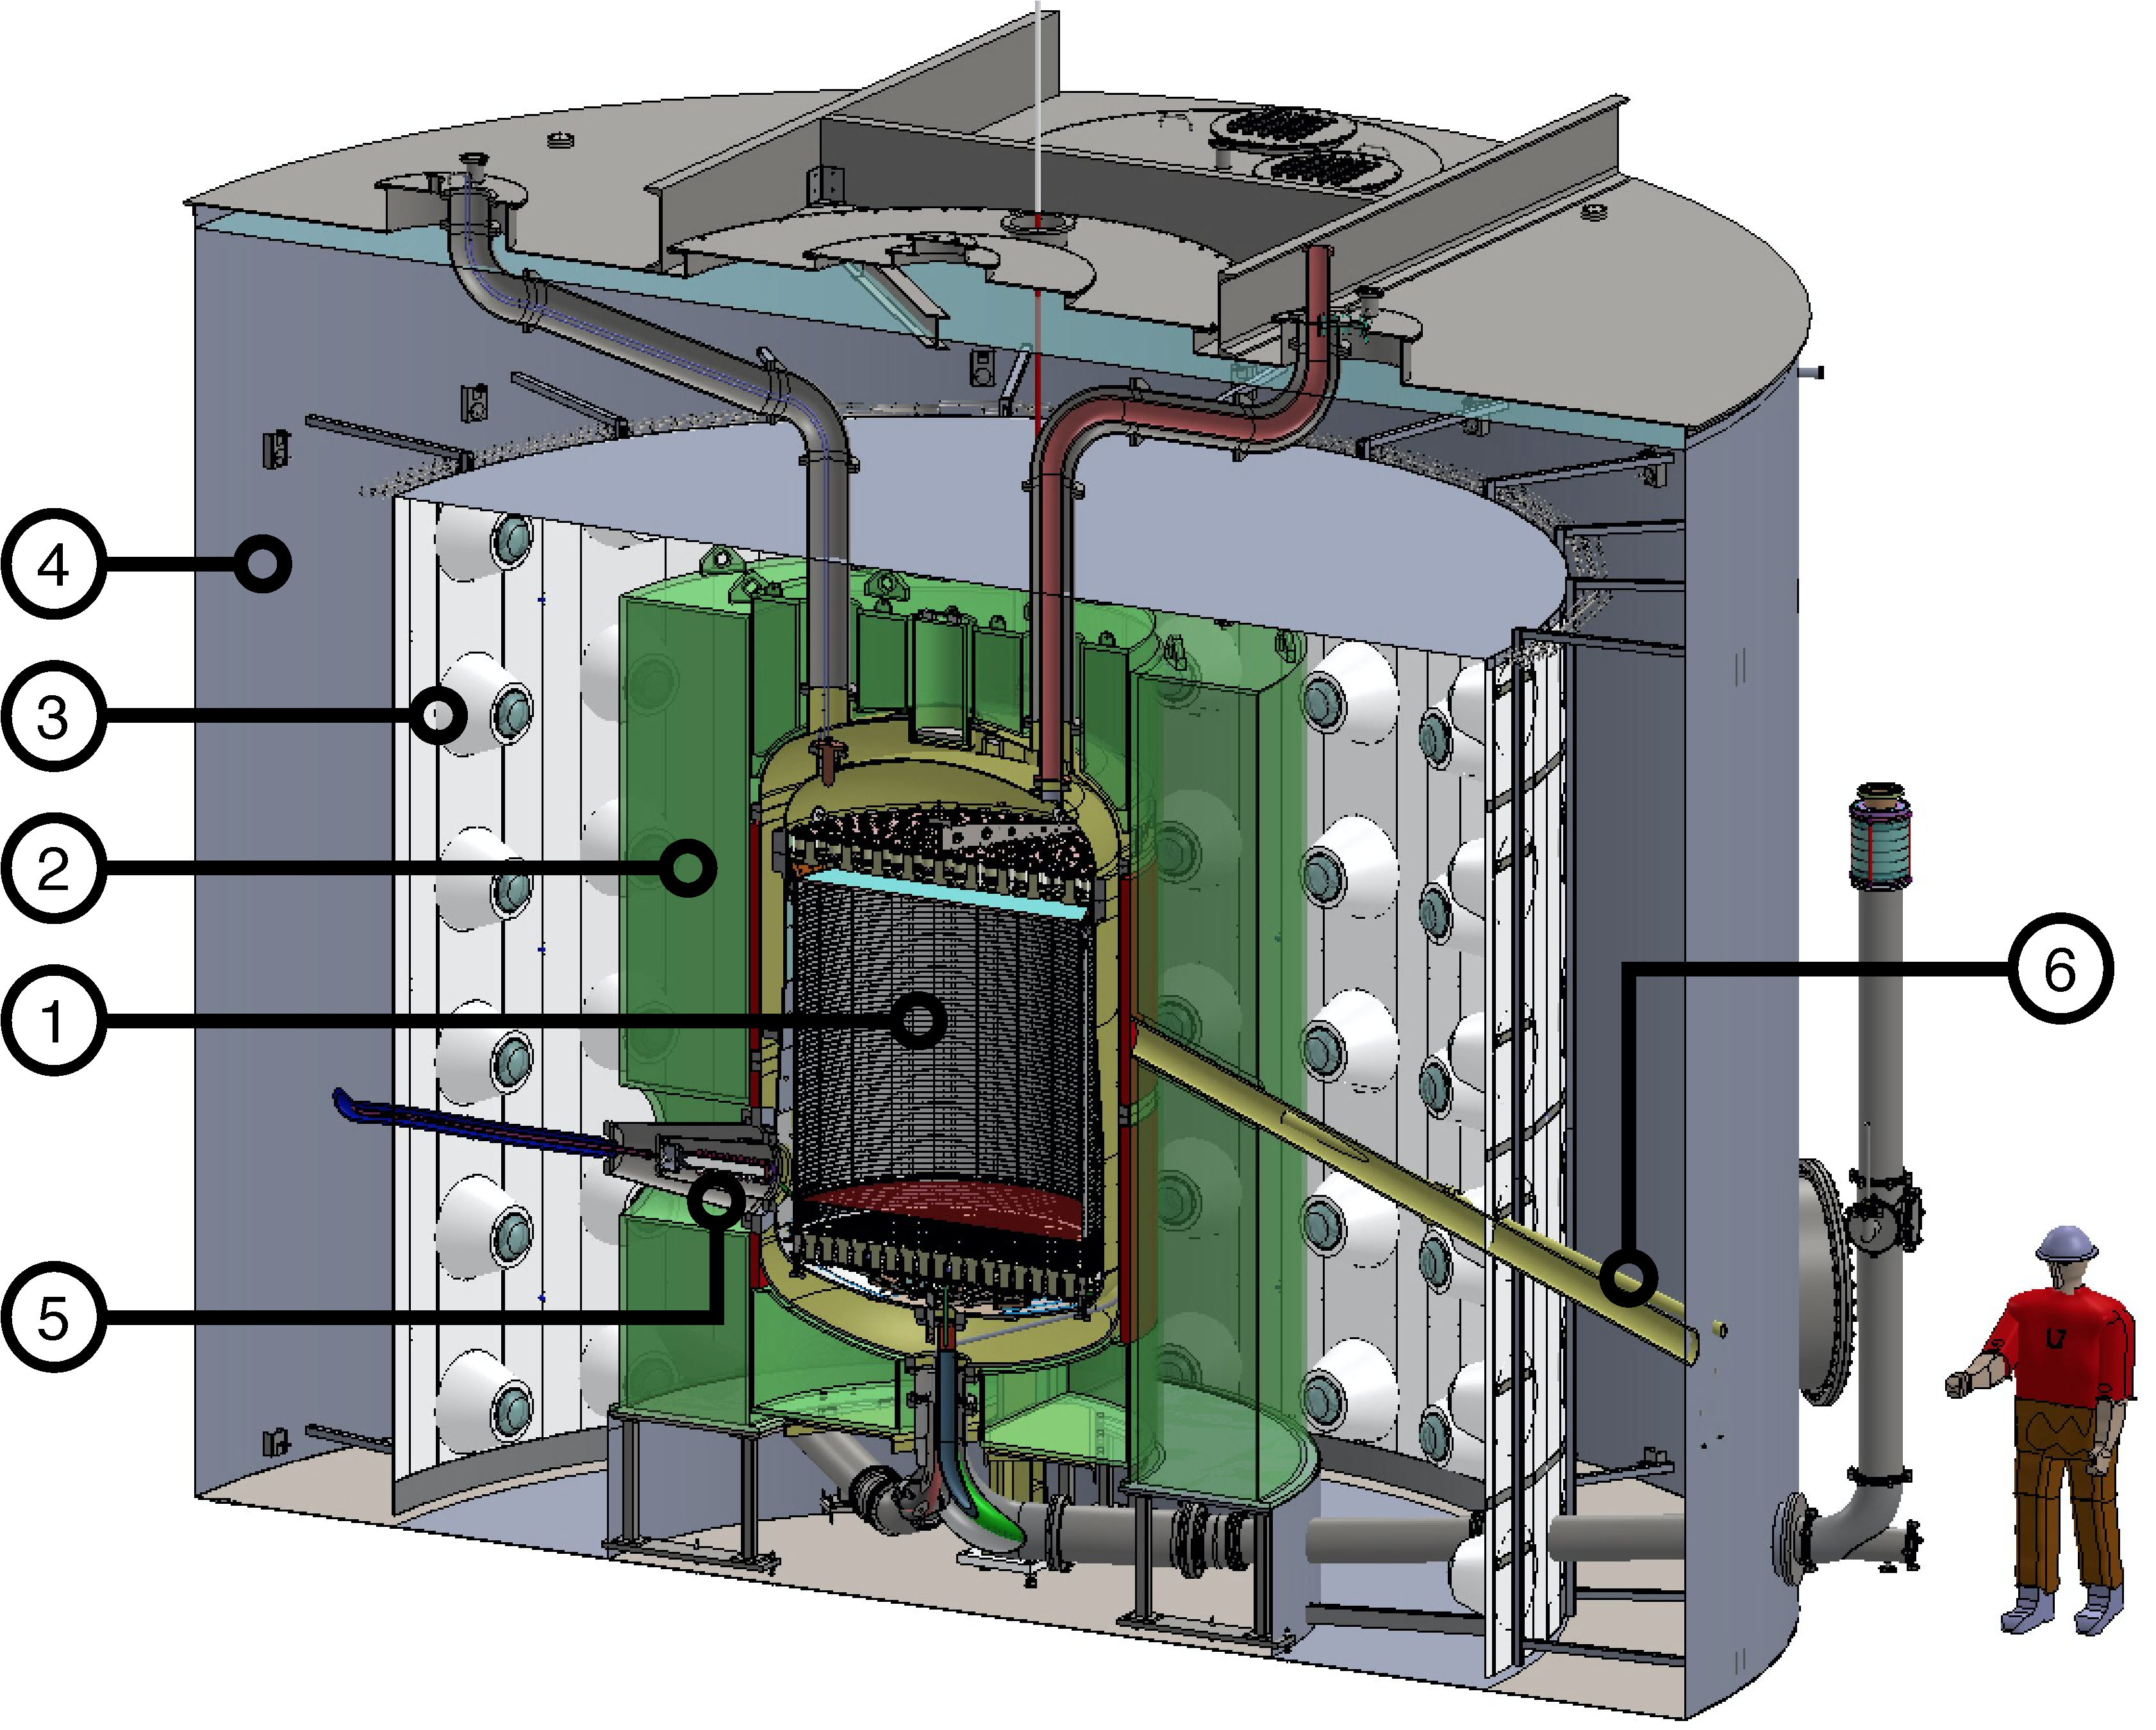
\includegraphics[width=0.7\linewidth]{figures/LZ/LZSchematic.pdf}
    \caption[Schematic of the LZ detector and its the major subsystems.]{Schematic of the LZ detector and its the major subsystems. At the centre is the liquid xenon TPC (1), monitored by two arrays of PMTs and serviced by various cable and LXe conduits (upper and lower). The TPC is contained in a double-walled vacuum insulated titanium cryostat and surrounded on all sides by a GdLS Outer Detector (2). The cathode high voltage connection is made horizontally at the lower left (5). The GdLS is observed by a suite of 8” PMTs (3) standing in the water (4) which provides shielding for the detector. The pitched conduit on the right (6) allows for neutron calibration sources to illuminate the detector \cite{LZNIMA}.}
    \label{fig:LZ/LZDetector}
\end{figure}
\section{Liquid xenon time projection chamber}\label{sec:LZ/LXeTPC}
The LZ TPC holds 7~t (5.6~t fiducial) of LXe above its cathode, there is an additional thin layer (8~mm thick) of gaseous xenon (GXe) at the top of the liquid. The active volume measures approximately 1.5~m in height and diameter and the walls of the TPC are made from PTFE to improve light collection efficiency \cite{LZNIMA}. The TPC, Skin and Xe payload are housed within the Inner Cryostat Vessel (ICV) and the Outer Cryostat Vessel (OCV) provides a vacuum jacket for insulation. Both cryostat vessels are made from low radioactivity titanium \cite{LZ:2017iwn}. When a particle scatters off a LXe atom a prompt scintillation signal (S1) is produced alongside free elections, via ionisation of the LXe atom. The free electrons are drifted to the LXe surface using an applied electric field and are extracted in the GXe layer. As the electrons accelerate through the GXe layer, a proportional amount of scintillation light (S2) is produced. Light produced from these particle interactions is observed by a top and bottom array of 3-inch Hamamatsu R11410–22 PMTs, 494 in total. Using both the S1 and S2 signals, position reconstruction techniques can be used to determine the $xyz$-position of the particle interaction. The time difference between the S1 and S2 signals combined with the drift velocity is used to determine the $z$-position of the interaction whilst the hit pattern of the S2 signal in the top PMT array provides $xy$-position. The operating principle of a TPC can be seen in \autoref{fig:LZ/TPCCartoon}, whilst the main components of the LZ TPC are shown in \autoref{fig:LZ/CAD_TPC}.
\begin{figure}[!ht]
    \centering
    \includesvg[width=0.9\textwidth]{figures/LZ/lz-event.svg}
    \caption{Schematic of a TPC with an event with a S1 and S2 pulse. Each particle interaction with the LXe atoms produces two signals: an initial prompt scintillation (S1) and a second, delayed one from ionisation (S2). The combination of these two signals allows for precise 3D position reconstruction and discrimination between nuclear and electron recoils. Original image courtesy of C. Faham and D. Malling.}
    \label{fig:LZ/TPCCartoon}
\end{figure}

\begin{figure}[!ht]
     \centering
     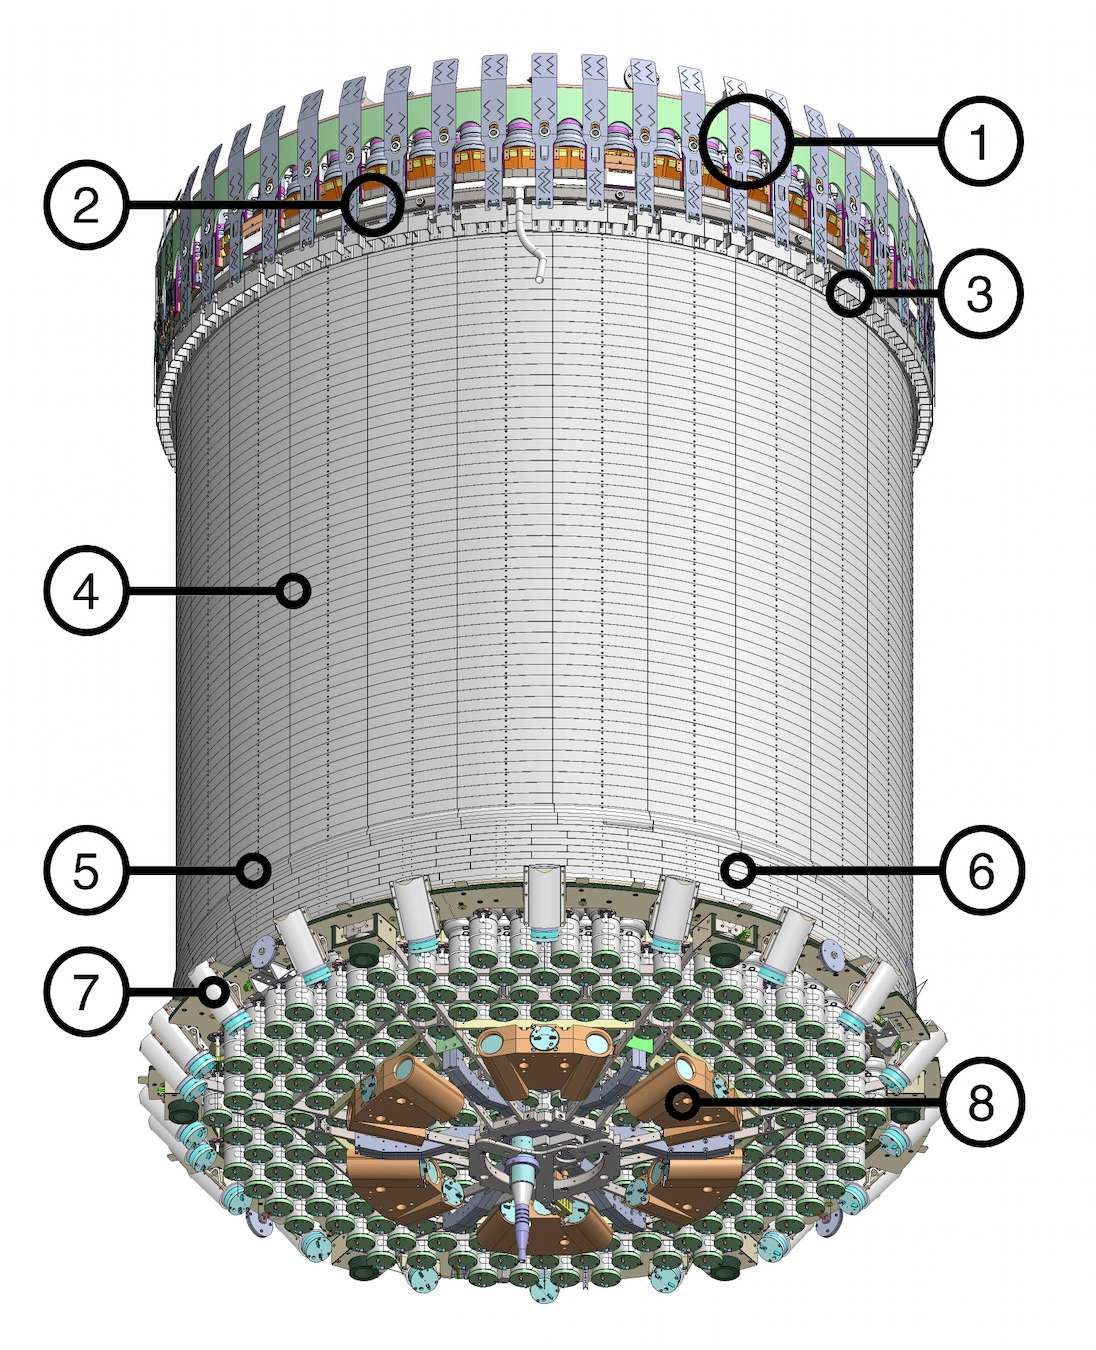
\includegraphics[width=0.5\textwidth]{figures/LZ/CAD_TPC.jpg}
     \caption{Drawing of the TPC \& Skin components: 1-Top PMT array; 2-Gate-anode and weir region (liquid level); 3-Side skin PMTs (1-inch); 4-Field cage; 5-Cathode ring; 6-Reverse field region; 7-Lower side skin PMTs (2-inch); 8-Dome skin PMTs (2-inch) \cite{LZNIMA}.}
     \label{fig:LZ/CAD_TPC}
\end{figure}

\subsection{Particle-Xenon interactions within a TPC}\label{sec:LZ/XeInteractionsTPC}
As a particle traverses the LXe volume it can interact with either the atomic nucleus, producing a nuclear recoil (NR), or with the surrounding electron cloud, producing an electronic recoil (ER). Both processes result in the pair of signals discussed in \autoref{sec:LZ/LXeTPC}. The S1 signal is produced via the following mechanism. The excited Xe atom, Xe$^{*}$, combines with a nearby ground state Xe atom to form an excimer state, Xe$_{2}^{*\nu}$, which is both an electronically and vibrationally excited molecule. Through collisions with other Xe atoms, energy in the vibrational modes of the excimer is lost. The excited pair de-excite further as the electronic excitation energy is released as a pair of vacuum-ultraviolet (VUV), at a mean wavelength of 178~nm \cite{Schumann:2014uva}.
The Xe atom also undergoes ionisation due to the displacement of the nucleus during the collision releasing electrons. A positively charged Xe$^{+}$ ion combines with a neutral Xe atom to form a positively charged dimer Xe$^{+}_{2}$. Most of the electrons that are emitted in the ionisation are drifted away from the collision site by the applied electric field. However some of the ionised electrons produced in the cascade recombine with the molecule prior to it splitting to form a highly excited Xe atom. A final series of relaxation occurs in a similar manner to the excitation luminescence excimer. A schematic which describes the process of producing the S1 and S2 signal can be seen in \autoref{fig:LZ/XenonSigalProduction}.
\begin{figure}[!ht]
    \centering
    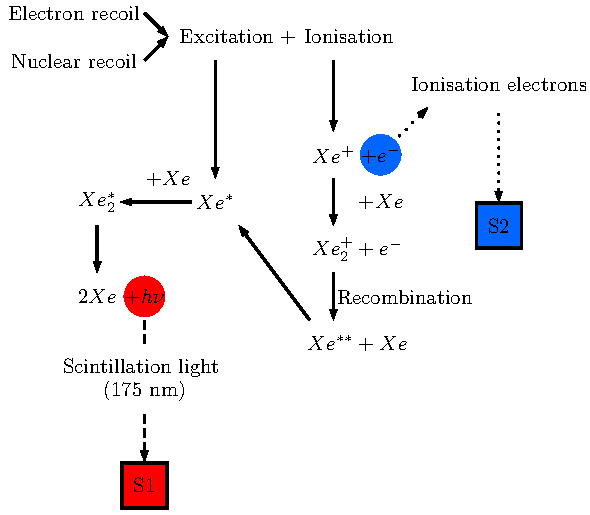
\includegraphics[width=0.7\linewidth]{figures/LZ/Xenon_interaction.pdf}
    \caption{A schematic of the signal production and collection in a dual phase xenon time projection chamber.}
    \label{fig:LZ/XenonSigalProduction}
\end{figure}
To understand what particle has passed through the LXe it is important to determine the energy deposited in interaction with the Xe atom. This can be described using the following equation:
\begin{equation}
    E=\frac{W}{L}(n_{ex}+n_{i})
    \label{eqn:EnergyRec_noG}
\end{equation}
Where $W$ is the average energy required to produced either one scintillation photon or ionisation electron, which has been measured to be $13.7\pm0.4$~eV \cite{Goetzke:2016lfg, Dahl:2009nta}.
$L$ is referred to as the "Lindhard factor" or "quenching" accounting for the reduction of produced light and charge as energy is lost to heat. For electron recoils $L$ is taken as unity, this implies that the heat-loss is constant with energy allowing it to be absorbed into the value of $W$ \cite{Rischbieter:2022}. The Lindhard factor for nuclear recoils is observed to be a function of deposited energy as the interaction energy is not linearly related to the observed total quanta \cite{Sorensen:2011bd}.
$n_{ex}$ and $n_{i}$ represent the number of excited atoms and ionised atoms respectively and are proportional to pulse area of the S1 and S2 pulses observed in the TPC respectively. The constants of proportionality are $g_1$ and $g_2$ and represent the S1 light collection efficiency and the electron extraction efficiency of the detector respectively. Thus \autoref{eqn:EnergyRec_G} can be modified to describe the energy deposition using:
\begin{equation}
    E=\frac{W}{L}\bigg(\frac{S1}{g_1}+\frac{S2}{g_2}\biggl)
    \label{eqn:EnergyRec_G}
\end{equation}

\subsection{NR and ER discrimination}\label{LZ/NRERDiscrim}
The ratio of of light to charge produced differs between NRs and ERs. This can be directly observed through the S1 and S2 pulse areas produced from the interactions, particularly the ratio, $\text{log}_{10}(\text{S2})/\text{S1}$. This method demonstrates 95\% discrimination against ER with a 50\% NR acceptance \cite{lzSens}. This is key in the search for WIMPs where we would expect to observe an NR when a WIMP passes through the TPC. However, the dominant backgrounds such as $\beta$-decays from Rn daughter isotopes and \textsuperscript{85}Kr and $\gamma$ radiation from detector components all produce ER events in the LXe. Both ER and NR events form distinctive band structure in $\text{log}_{10}(\text{S2})/\text{S1}$ space, as shown in \autoref{fig:LZ/NRERBandExample}, where the width of the bands is due to electron-ion recombination at the interaction site whilst the overall separation is due to the ratio of ionisation to excitation in the interaction \cite{Dahl:2009nta}.

\begin{figure}[!ht]
    \centering
    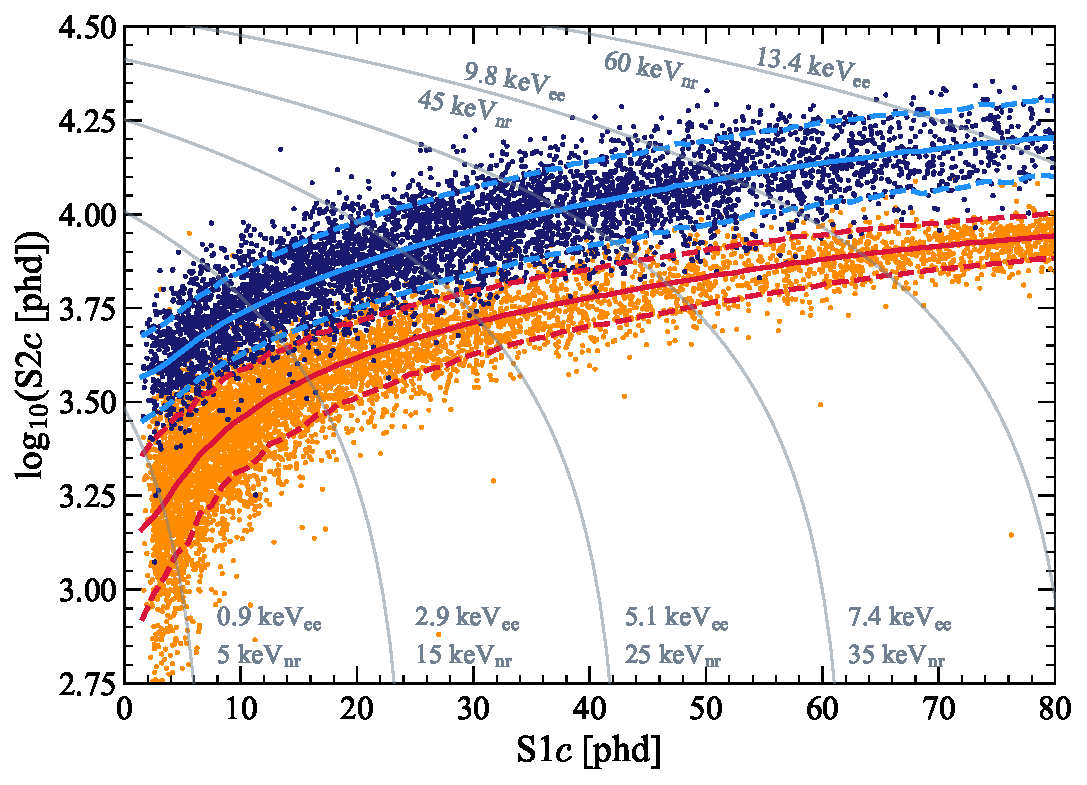
\includegraphics[width=0.7\linewidth]{figures/LZ/SR1WS_calOnly_0629.pdf}
    \caption[Discrimination between ER and NR in LZ using calibration events.]{Discrimination between ER and NR in LZ using calibration events in $\text{log}_{10}\text{S2}_{\text{c}}/\text{S1}_{\text{c}}$ for the tritium source (dark blue points, 5343 events) and the DD neutron generator (orange points, 6324 events). Solid blue (red) lines indicate the median of the ER (NR) simulated distributions, and the dotted lines indicate the 10\% and 90\% quantiles. The thin gray lines represent contours of constant electron-equivalent energy (keV$_{\text{ee}}$) and nuclear recoil energy (keV$_{\text{nr}}$) \cite{LZ:2022lsv}.}
    \label{fig:LZ/NRERBandExample}
\end{figure}

\section{Xenon Skin}\label{sec:LZ/Skin}
The TPC is surrounded by a layer of LXe, the region contains around 2~t of LXe between the field cage and the inner cryostat vessel \cite{LZNIMA}. The primary motivation for including this layer of LXe was to provide dielectric insulation between the two elements. Unlike XENONnT, LZ's main competitor, this region is instrumented for optical readout acting as a scintillation-only veto detector for gamma ray interactions in the TPC~\cite{XENON:2024wpa}. The region is known as the "Skin" and can be divided into two regions: Barrel and Dome. The Barrel contains 93 1-inch Hamamatsu R5820 PMTs at the top of the Barrel looking down and 38 2-inch Hamamatsu R8778 PMTs; 20 at the bottom of the Barrel looking up, and 18 in the Dome region below the TPC \cite{LZNIMA}. The layout of the Skin PMTs with respect to the TPC can be seen in \autoref{fig:LZ/CAD_TPC}.

\section{Outer Detector}\label{sec:LZ/LZOD}
It has been shown in previous sections that dual phase TPC has the capability to distinguish between ER and NR interactions in the LXe, however it does not have the capability to determine what particle caused the recoil. Neutrons are the primary source of NRs as they scatter off the Xe nuclei and mimic a signal similar to a WIMP. Neutrons are likely to scatter multiple times in the TPC and OD whereas WIMPs would scatter only once due to differences in their respective interaction cross sections. LZ is taking advantage of this principle by surrounding the TPC with a neutron detector to increases the discrimination against NR backgrounds. This detector is the Outer Detector.
%and together with the Xe Skin comprises the LZ Veto System. 
The outer cryostat housing the TPC is surrounded near hermetically by ten acrylic vessels filled with  Gadolinium loaded liquid scintillator (GdLS). The GdLS is observed by 120 PMTs and surrounded by 238~t of DI water which provides additional shielding to the detector and can be used to detect muons which emit Cherenkov radiation as they pass through the water. An exploded view of these vessels can be seen in \autoref{fig:LZ/ODTanks}.
\begin{figure}[!ht]
    \centering
    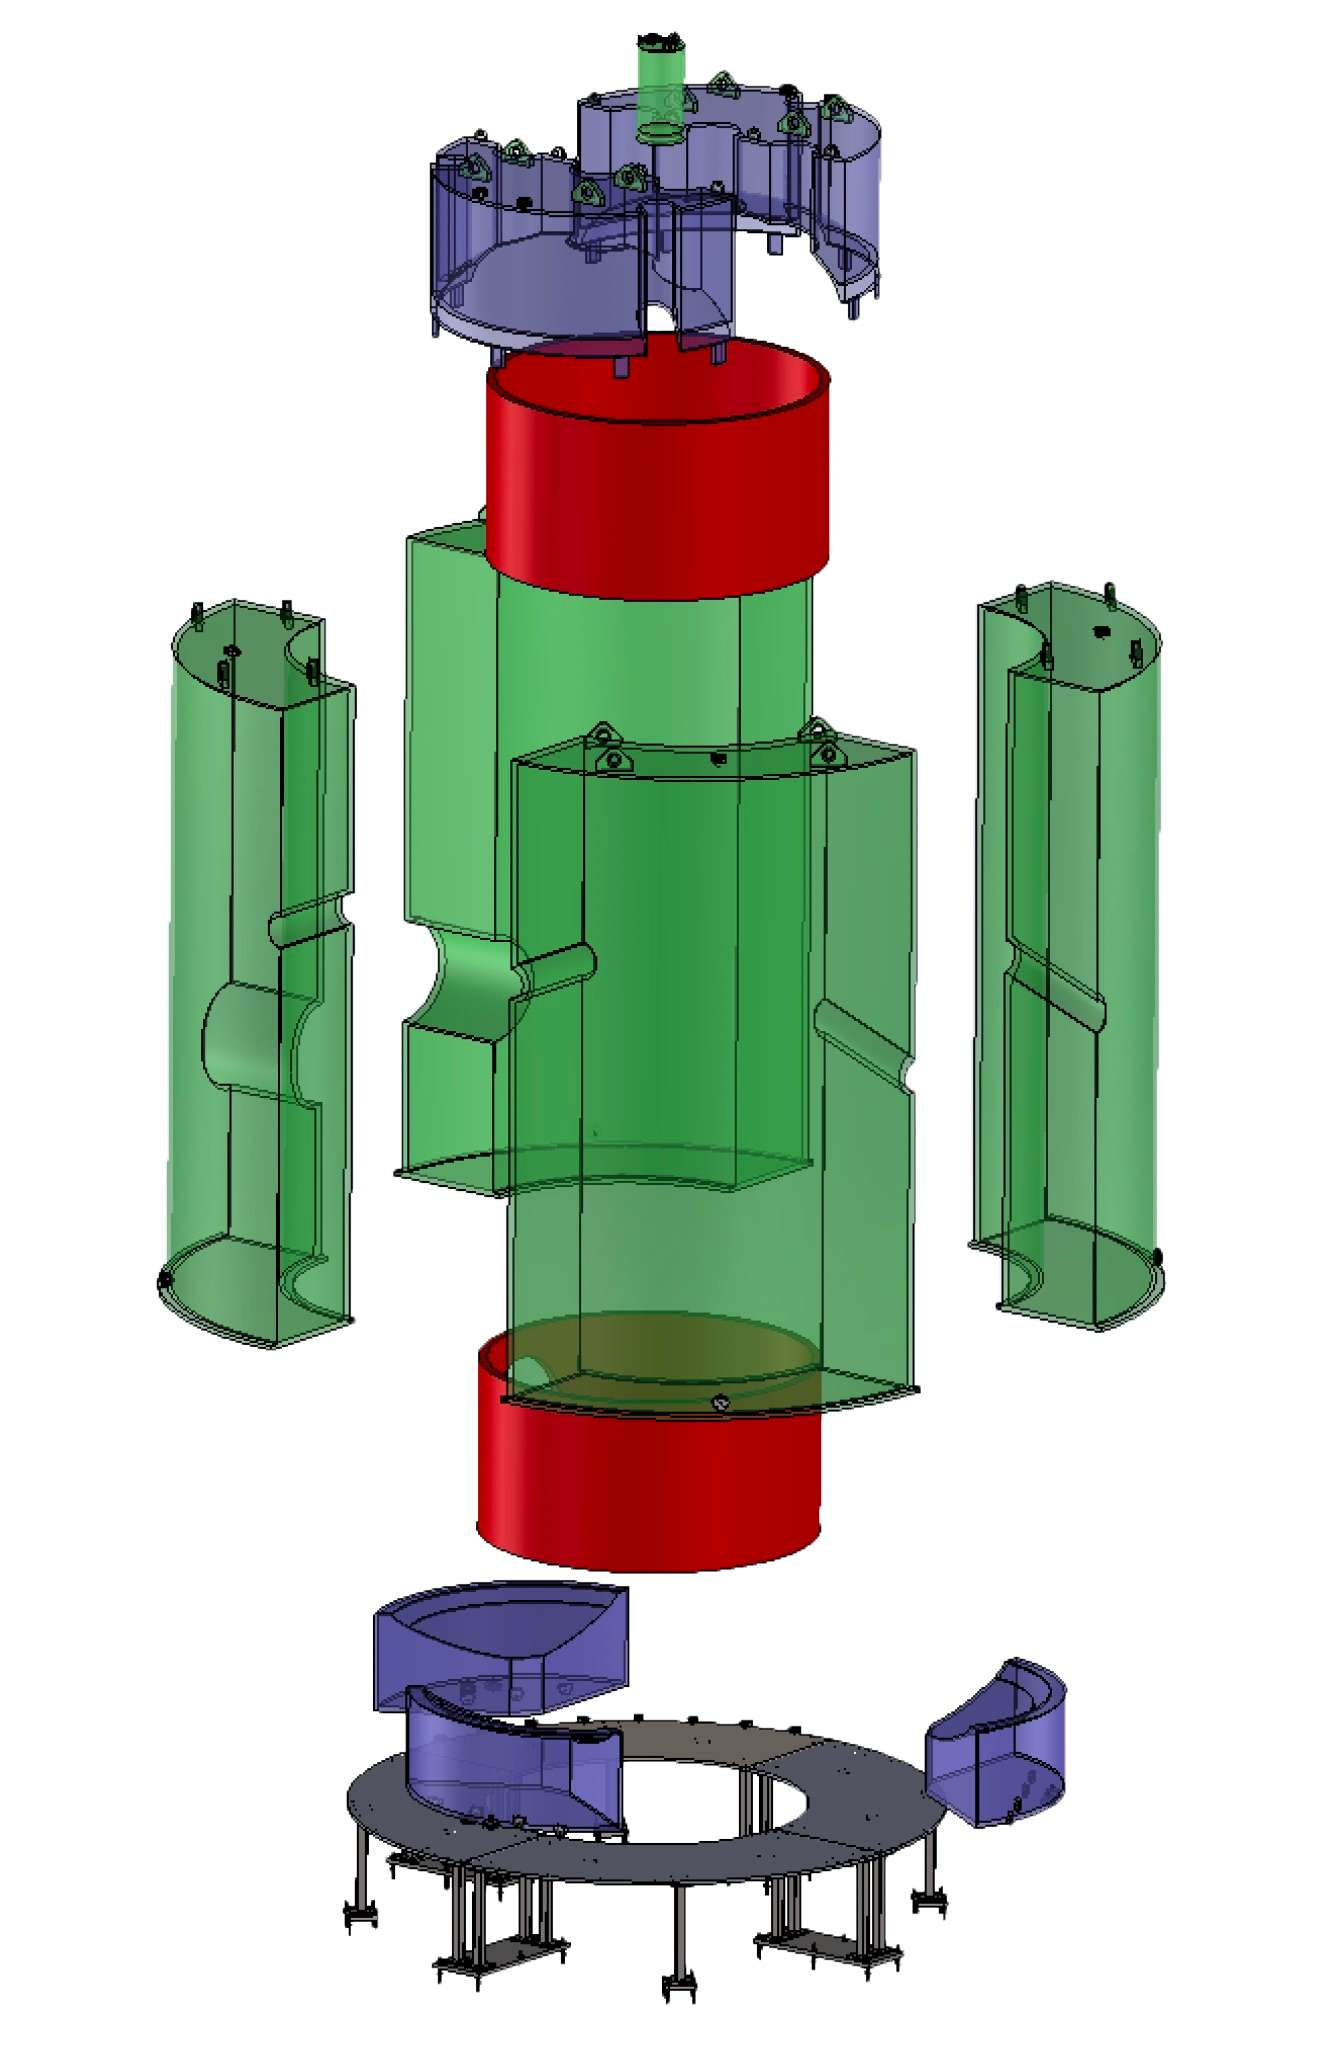
\includegraphics[width=0.5\linewidth]{figures/LZ/CAD_ODTanks.jpg}
    \caption{The Outer Detector vessels in an exploded view. The four large side vessels (SATs) are shown in green, the five small vessels (two top (TATs) and three bottom (BATs)) are shown in blue. The stainless steel base is given in grey and the foam water displacers in red. There is an additional small vessel shown in green at the top which is removed for photo-neutron calibration source deployment \cite{LZNIMA}.}
    \label{fig:LZ/ODTanks}
\end{figure}

\subsection{Liquid scintillator}\label{sec:LZ/LS}
The primary detection medium for the OD is the GdLS, chosen for its excellent efficiency for neutrons and gammas that reach the OD \cite{LZTDR}. The composition of the GdLS mixture is shown in \autoref{tab:LZ/GdLSComp}. The base of the LS mixture is Linear-alkylbenzene (LAB), which acts as a solvent for the other components of the mixture. In addition to the LAB, the fluor 2,5-diphenyloxazole (PPO), and the wavelength shifter 1,4-bis(2-methylstyryl(benzene)) (Bis-MSB) are considered as the LS. As particles pass through the LS, the LAB component is excited as the particles deposit energy along the tracks. Through a series of chemical reactions, the excited LAB transmits energy to the fluor. As the excited fluor de-excites, it emits light with wavelengths up to 380~nm. Due to the short absorption lengths of the LS below 380~nm (approximately 1~m), Bis-MSB is included as a wavelength shifter. The Bis-MSB absorbs the photons produced by the fluor and emits photons with wavelengths between 410~nm~-~425~nm with absorption lengths over 10~m. Bis-MSB is a crucial component of the mixture as wavelengths of the emitted photons overlap with the PMT sensitivity spectrum and absorption lengths satisfy the detector geometry.
The mixture is additionally loaded with Gd with a mass fraction of 0.1\%. Gd has a very high $(n,\gamma)$ cross-section so improves both the efficiency and intensity of the neutron capture signal \cite{LZTDR}. Due to the effectiveness of the Gd, only a small mass fraction is needed to dominate over neutron capture on protons in the LS. To dissolve the Gd in solution with the LS it is bound to a chelating agent, 3,5,5-trimethylhexanoic acid (TMHA) in a 3:1 ratio \cite{LZTDR,Haselschwardt:2018vmp}.
\begin{table}[!ht]
    \centering
    \caption{Chemical components in 1L of GdLS, adapted from Ref.~\cite{Haselschwardt:2018vmp}.}
    \begin{tabular}{llll}
        \hline\hline
        \textbf{Component} & \textbf{Molecular Formula} & \textbf{Mass [g/L]} & \textbf{Mass Fraction} \\
        \hline
        LAB & $\text{C}_{17.14}\text{H}_{28.28}$ & 853.55 & 99.25\\
        PPO & $\text{C}_{15}\text{H}_{11}\text{NO}$ & 3.00 & 0.35 \\
        bis-MSB & $\text{C}_{24}\text{H}_{22}$ & 0.01 & 0.0011\\
        TMHA & $\text{C}_{9}\text{H}_{17}\text{O}_{2}^{-}$ & 2.58 & 0.003\\
        Gd & Gd & 0.86 & 0.1 \\
        \hline
        GdLS & $\text{C}_{17.072} \text{H}_{28.128} \text{O}_{0.0126} \text{N}_{0.0037} \text{Gd}_{0.0015}$ & 860.00 & 100 \\
        \hline\hline
    \end{tabular}
    \label{tab:LZ/GdLSComp}
\end{table}
\subsubsection{Neutron capture in the OD}\label{sec:LZ/NeutronCapture}
As previously mentioned, Gadolinium has the largest capture cross-section for thermal neutrons of any known stable elements: 49~kb \cite{Hagiwara:2018kmr}. This is due to contributions of two isotopes $^{155}\text{Gd}$ (61~kb) and especially $^{157}\text{Gd}$ (254~kb) \cite{Hagiwara:2018kmr}. After a thermal neutron captures on $^{157}\text{Gd}$, the $^{158}\text{Gd}^*$ compound nucleus remains in a 7837 keV excited state, a subsequent de-excitation occurs via a cascade of on average 4-5 $\gamma$-ray emissions \cite{Hagiwara:2018kmr}. The de-excitation is illustrated in \autoref{fig:LZ/Gd158Deexcite}. The continuum component of the $\gamma$-ray spectrum see in \autoref{fig:LZ/ODEnergySpec} is depicted in \autoref{fig:LZ/Gd158Deexcite} where the multi-step de-excitations of $^{158}\text{Gd}^*$ can occur between unresolvable levels in quasicontinuum (dashed lines), within discrete levels (solid lines). This results in a random distribution of both the number and energy of the emitted $\gamma$-rays. 

\begin{figure}[!ht]
    \centering
    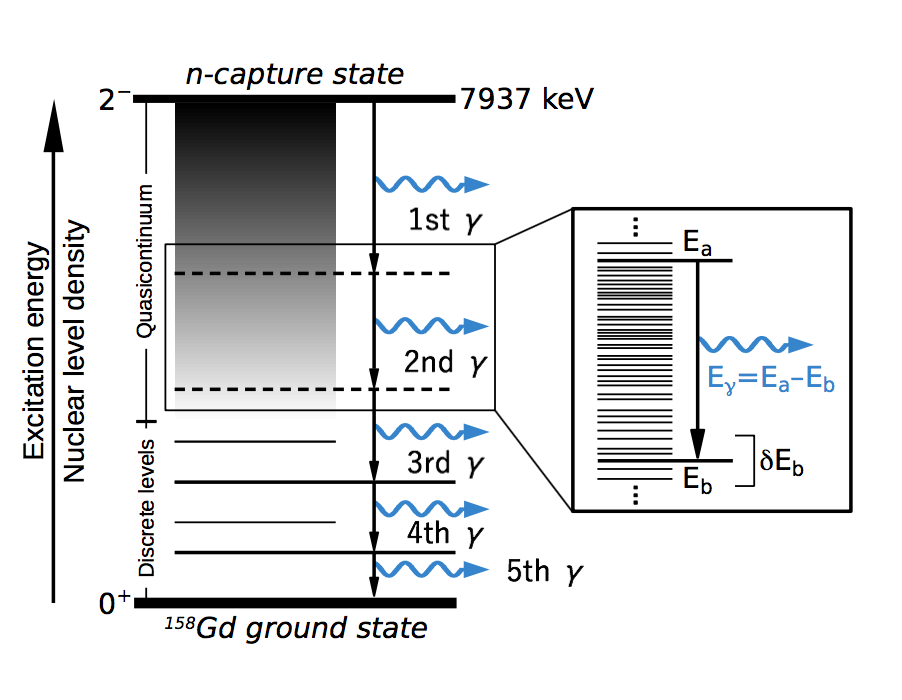
\includegraphics[width=0.7\linewidth]{figures/LZ/ContinuumEmission2.png}
    \caption{Illustration of the multi-step $\gamma$-ray emission of an excited $^{158}\text{Gd}^*$ following the thermal $^{157}\text{Gd}(n,\gamma)$ reaction. The de-excitation to the ground state can occur via many intermediate levels. Adapted from Ref.~\cite{Hagiwara:2018kmr}.}
    \label{fig:LZ/Gd158Deexcite}
\end{figure}
In addition to neutron capture of Gd, hydrogen also produces a neutron capture signal. Hydrogen has thermal neutron capture cross section of 0.33~b which appears meagre in comparison with Gd, however due to the abundance of hydrogen in the LS, acrylic, and water, a significant number of neutron captures are observed. Following the capture of a thermal neutron, the excited deuterium atom decays to its ground state and emits a single 2.2~MeV $\gamma$-ray \cite{LZTDR}. The prominent peak resulting from the hydrogen capture can be seen in the OD energy spectrum shown in \autoref{fig:LZ/ODEnergySpec}.
\begin{figure}[!ht]
    \centering
    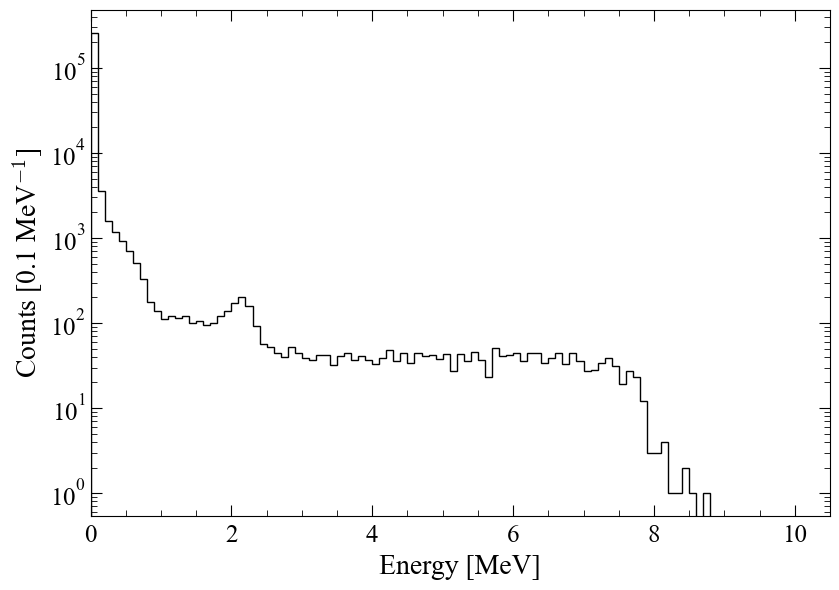
\includegraphics[width=0.7\linewidth]{figures/LZ/ODEnergySpec.png}
    \caption{AmLi energy spectrum measured with LZ Outer Detector with coincident single scatter signals in the TPC, here simple data quality cuts have been applied. The distinctive hydrogen capture peak can be seen at 2.2~MeV, whilst the continuous $\gamma$-ray spectrum from the Gd Capture has the expected end point at $\mathtt{\sim}$8~MeV.}
    \label{fig:LZ/ODEnergySpec}
\end{figure}
By doping LS with Gd, the efficiency for detecting at least one of the capture gammas is very high compared to having pure LS. Another advantage of Gd-doping is reduction in the time delay for neutron capture from 220~\textmu s to 28~\textmu s intern reducing the length of the window needed for vetoing by a factor of 7 \cite{LZTDR}. Detailed simulations by the LZ Collaboration initially expected to use a veto window of 125~\textmu s, however it was found that neutrons also captured in the acrylic up to 10\% of the time \cite{LZTDR}. Further studies by the author also found that neutrons captured in the water which had partially saturated foam displacer between the acrylic tanks and OCV. This effect further extended the required veto window to 600~\textmu s. This study is discussed further in \autoref{sec:VetoEff/NCT}.

\subsection{PMT system}\label{sec:LZ/ODPMTs}
Interactions in the GdLS and water are monitored by 120 Hamamatsu 8-inch R5912 photo-multiplier tubes (PMTs) arranged as shown in \autoref{fig:LZ/ODPMT_Array}. 
This model of PMT has been used successfully prior to their use in LZ at Daya Bay whose detector design is echoed in the LZ OD design \cite{Cao:2016vwh}. The R5912 PMTs were chosen because of the following reasons:
\begin{enumerate} 
    \item The spectral response ranges from 300~nm to 650~nm, with a peak wavelength at 420~nm. This encompasses the range of the scintillation light from the LAB mix between 390~nm to 440~nm \cite{Haselschwardt:2018vmp}. The comparison can be made comparing the plots in \autoref{fig:LZ/ODPMTSpecRes}.
    \item The quantum efficiency covers the relevant range, with an average expected value of $\sim25\%$ at 430~nm, as shown in \autoref{fig:LZ/ODPMTQE}.
    \item The radioactivity levels of the PMTs and support structure is a fairly weak constraint due to the 84~cm of water separating them from any active volume. In the scintillator itself, the simulated event rate from the PMT radioactivity is $<4~\text{Hz}$ \cite{LZTDR}. 
\end{enumerate}
\begin{figure}[!ht]
    \centering
    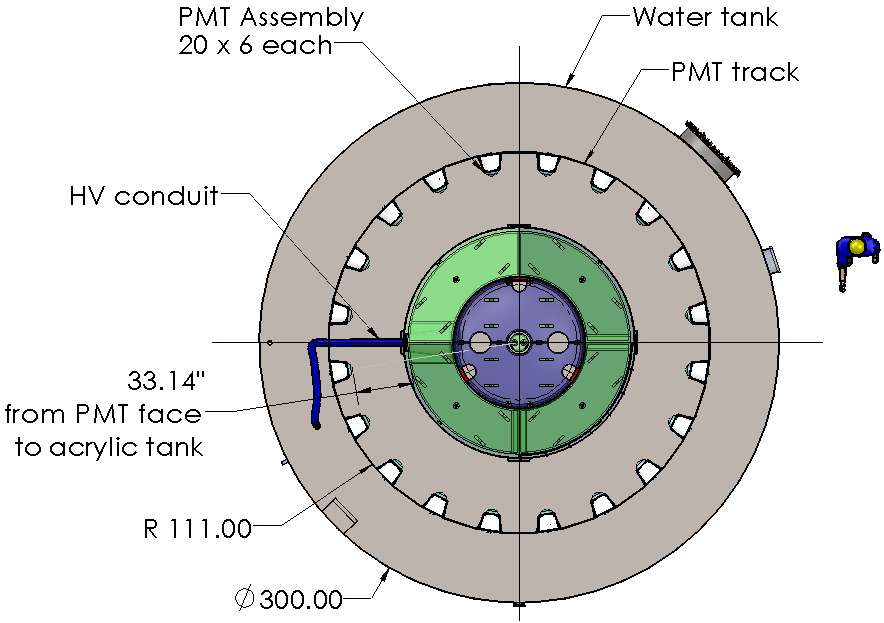
\includegraphics[width=0.7\linewidth]{figures/LZ/OD_PMT_support.jpg}
    \caption{Plan view of the OD PMT support system. The 20 PMT ladders are mounted to a circular track attached to the walls of the water tank \cite{LZTDR}.}
    \label{fig:LZ/ODPMT_Array}
\end{figure}
\begin{figure}[!ht]
     \centering
     \begin{subfigure}{0.47\textwidth}
         \centering
         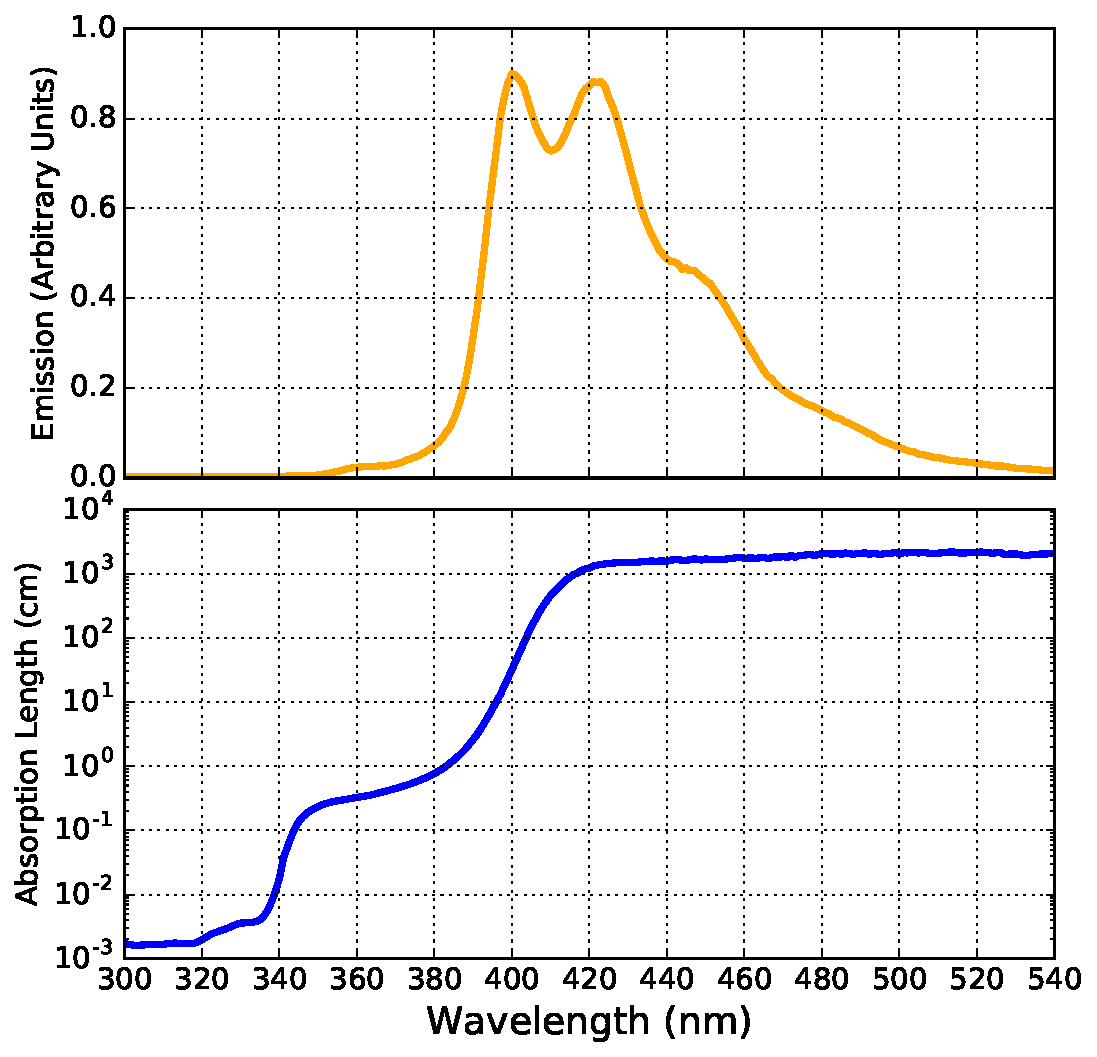
\includegraphics[width=\textwidth]{figures/LZ/GdLS_SpectralResponse.pdf}
         \caption{Wavelength dependence of two optical properties of the GdLS. \textbf{Top:} Emission spectrum of scintillation light. \textbf{Bottom:} The  absorption length of GdLS \cite{Haselschwardt:2018vmp}.}
         \label{fig:LZ/GdLSSpecRes}
     \end{subfigure}
     \hfill
     \begin{subfigure}{0.47\textwidth}
         \centering
         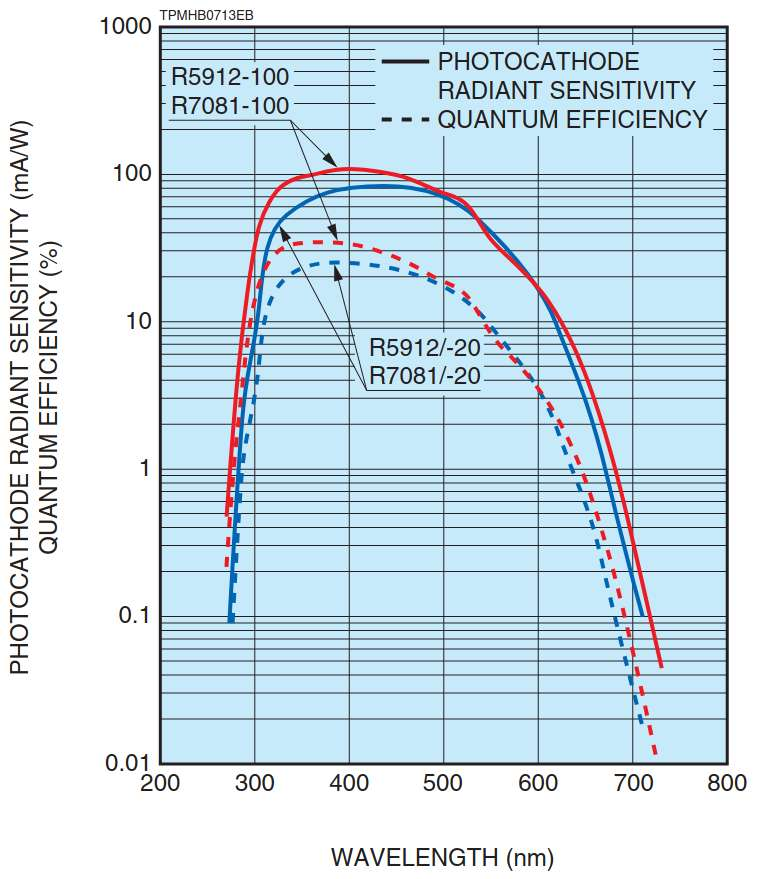
\includegraphics[width=\textwidth]{figures/LZ/ODPMT_QEvsWL.png}
         \caption{Wave length dependence of the quantum efficiency of the Hamamatsu 8-inch R5912 photo-multiplier tube. Adapted from Ref.~\cite{HamamatsuR5912}}
         \label{fig:LZ/ODPMTQE}
     \end{subfigure}
     \caption{A comparison of the wavelength dependence of key optical parameters for both the GdLS and PMTs.}
     \label{fig:LZ/ODPMTSpecRes}
\end{figure}
Prior to the installation of the PMTs at SURF, rigorous testing to fully characterise the response of tubes was carried out by groups from Brandeis University and the IBS Center for Underground Physics. Further details of the quality assurance testing is documented in Ref.~\cite{lkorley:thesis}.

\subsection{Outer detector optical calibration system}\label{sec:LZ/ODOCS}
LZ uses an optical calibration system to monitor: the PMT gain/single photoelectron (SPhE) size; afterpulsing rates; and the optical properties of the acrylic and scintillator. Light produced by the LED-driven system is injected into the OD at 35 different locations. Thirty injection points are evenly distributed throughout the PMT array  (10 azimuthal positions at 3 heights as shown in \autoref{fig:LZ/OCSPositions}). Four of the injection points are each positioned in centre of the side acrylic tanks facing upwards to monitor the optical properties of the GdLS. One final injection points is positioned in the outer rim of a side acrylic tank also facing upwards and is used to monitoring the optical properties of the acrylic.
\begin{figure}[!ht]
    \centering
    \includegraphics[width=0.9\linewidth]{figures/LZ/OD_PMT_CAD_picture_v4.png}
    \caption{\textbf{Left:} A cross-section of a CAD drawing of the OD. The three  heights of the 10 azimuthal positions of the optical fibre injection points are labelled 1-3. Two injection positions under the side acrylic tanks which point upwards are labelled 4 and 5. \textbf{Right:} A photograph of the OD PMT array showing the point of an injection point relatively to the surrounding PMTs.}
    \label{fig:LZ/OCSPositions}
\end{figure}
Duplex fibres are used to inject light pulses produced by LEDs to the different locations. For the thirty injection points situated within the PMT, 435~nm LEDs are used to match the peak wavelength and quantum efficiency of OD PMTs. Only one core in the fibre is used, the additional core is a backup in the event of any damage to the first core. LEDs with 435~nm and 450~nm wavelengths were chosen for the injection points facing into the LS to monitor optical degradation of the scintillator. Below 420~nm the absorption length of GdLS decreases significantly as shown in \autoref{fig:LZ/GdLSSpecRes}, if the scintillator degrades this region shifts to higher wavelengths. A similar approach is taken for monitoring the optical properties of the acrylic using 390~nm and 435~nm LEDs. The transmission of light through the acrylic varies with wavelength, as shown in \autoref{fig:LZ/AcrylicQA}. Monitoring the optical properties of the acrylic and scintillator during science runs is key to ensure consistent light collection during science runs.
\begin{figure}[!ht]
    \centering
    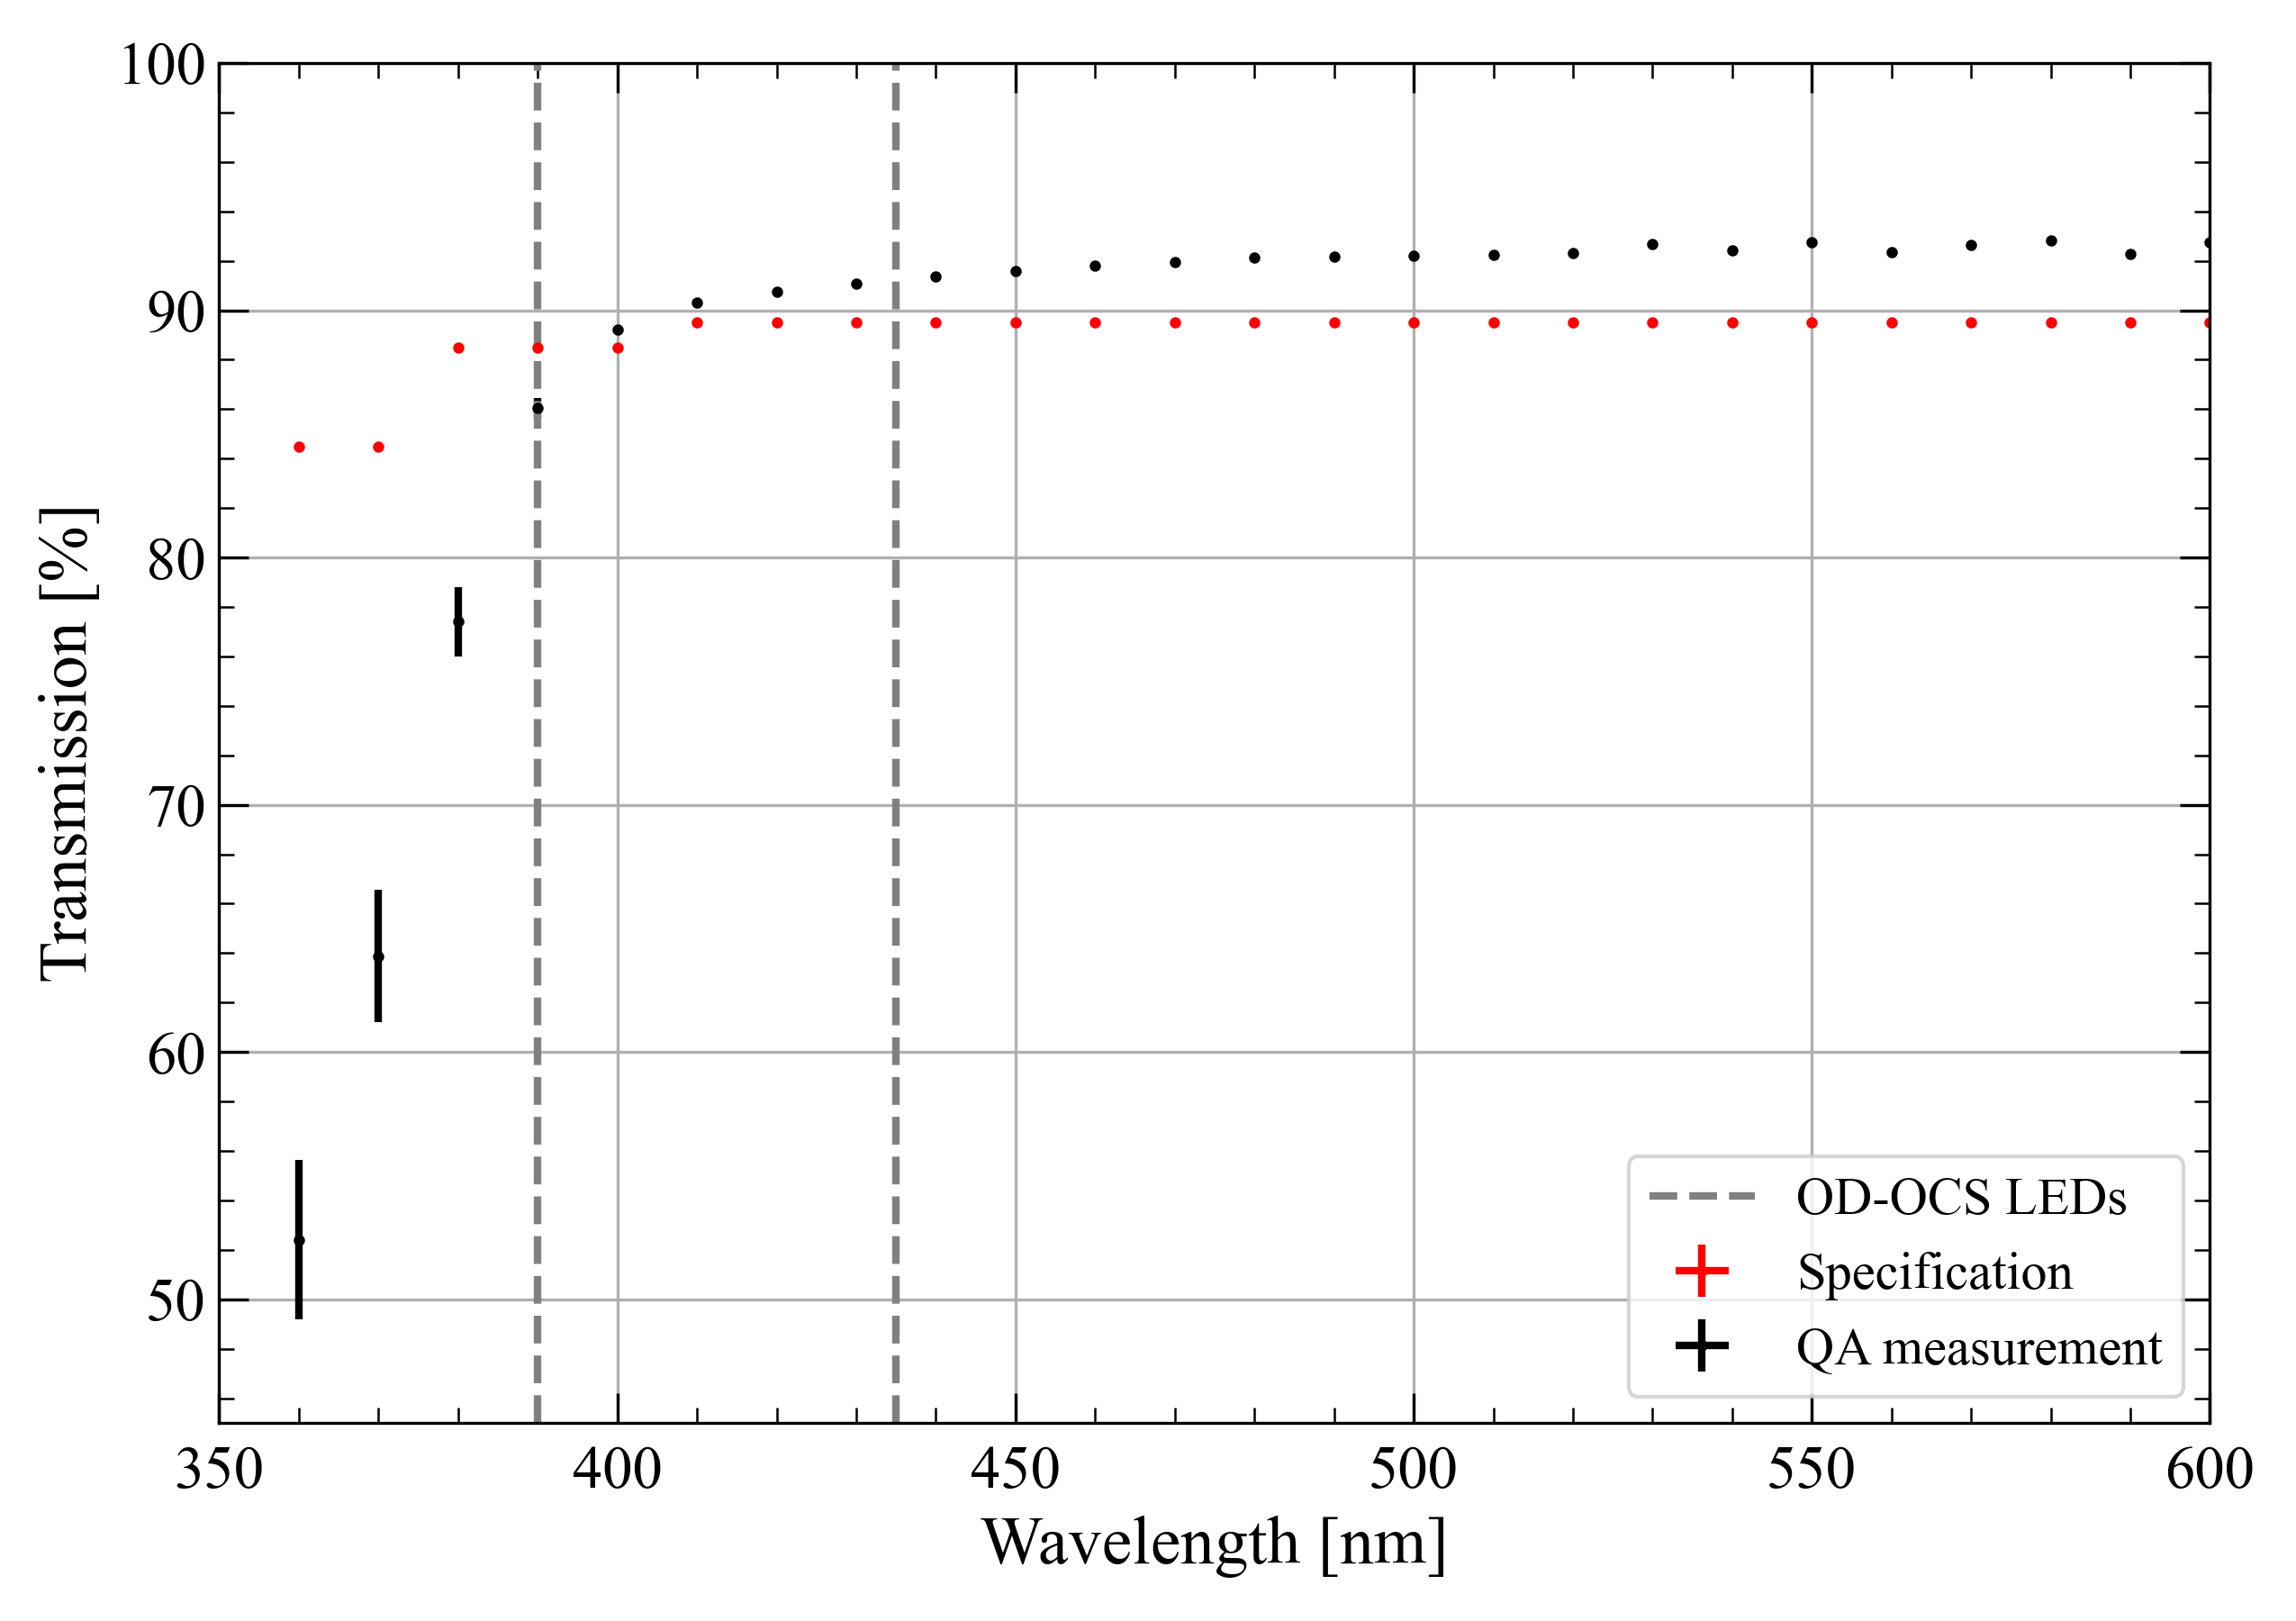
\includegraphics[width=0.7\linewidth]{figures/LZ/T187-XDM-UVT_WAVELENGHT_08252017.png}
    \caption{Quality assurance measurement data taken during the commissioning of the acrylic tanks. The QA measurement data is the average transmission of light at a particular wavelength across 46 points. Vertical lines indicate the 390~nm and 435~nm LEDs with respect to the transmission of light.}
    \label{fig:LZ/AcrylicQA}
\end{figure}
The electronics system which controls the LEDs consists of five Optical Calibration Cards (OCC). Each OCC consists of an FPGA controlled motherboard which houses eight LED pulser boards and two four-channel photodiode boards. Light pulses from the LEDs are divided by a three-way optical coupler: to the injection points in the OD; to the photodiode readout for onboard monitoring; to a monitoring PMT. The layout of the system can be seen in \autoref{fig:LZ/OCSSchematic}.
\begin{figure}[!ht]
    \centering
    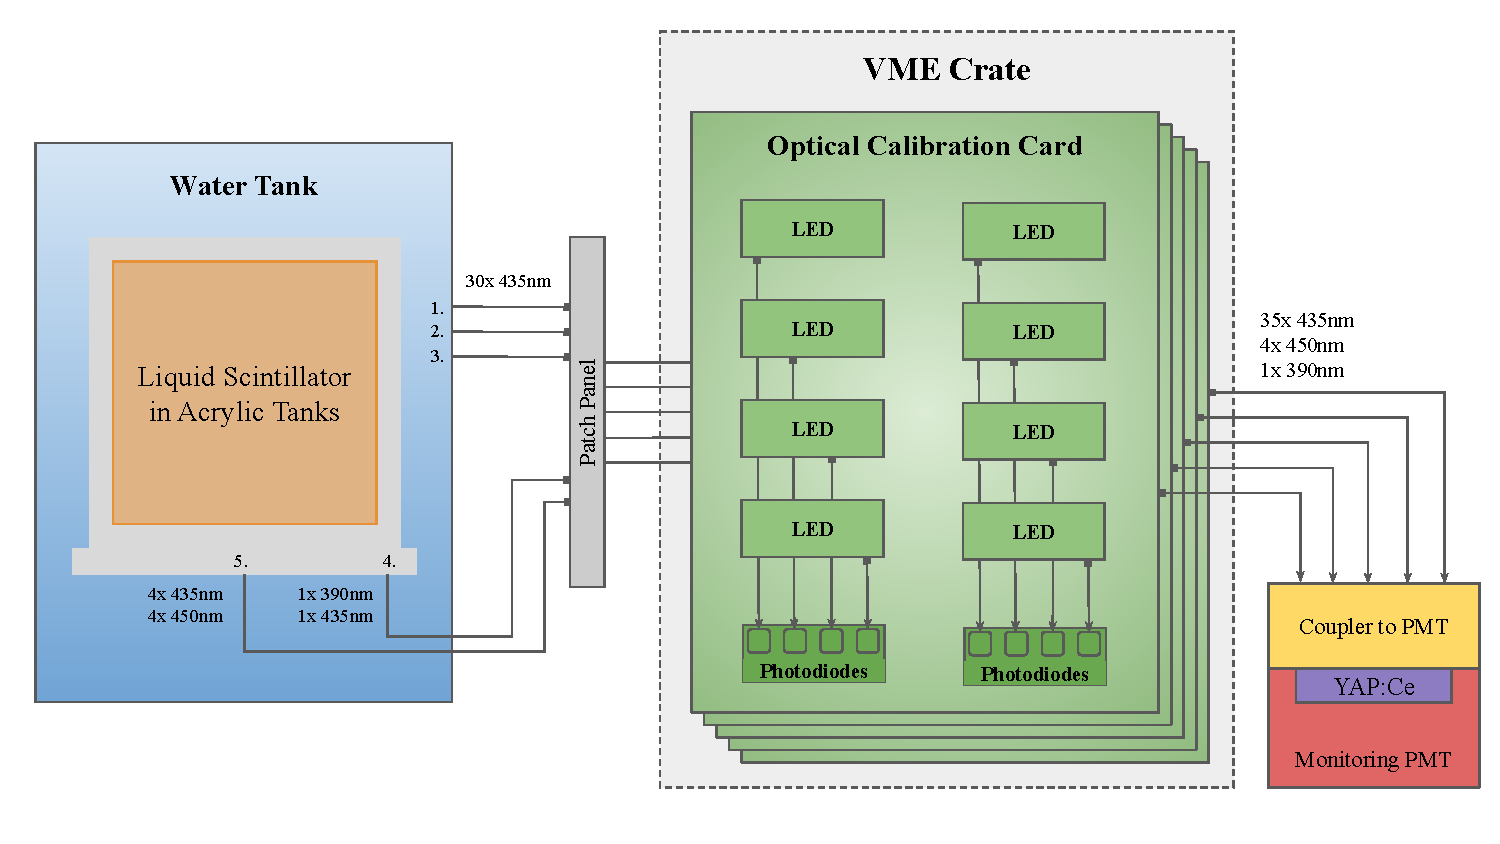
\includegraphics[width=0.9\linewidth]{figures/LZ/OCSSchematics.pdf}
    \caption{A schematic of the OD OCS. An example of one Optical Calibration Card (OCC) is shown with its eight LED pulser boards and two photodiode boards. A total of five OCCs make up the OCS and are powered by a VME crate. Lines with arrows show the paths light takes down various fibres to different positions in the system. Labels 1-3 represent the three heights within the PMT array, while Label 4-5 denote the injection points to monitor the GdLS/acrylic, as shown in \autoref{fig:LZ/OCSPositions}. Adapted from Ref.~\cite{Turner:2021qvi,LZ:2024bsz}.}
    \label{fig:LZ/OCSSchematic}
\end{figure}
The intensity of light is monitored using the onboard photodiode and rack mounted monitoring PMT, which is the same 8-inch Hamamatsu R5912 PMT as used in the OD PMT array \cite{Turner:2021qvi}. The commissioning of this component of the subsystem is covered further in \autoref{chap:ODCommissioning}. The OCS is controlled through LZ's central Slow Control System, allowing a user to define a pulse size/intensity using a graphical user interface \cite{hbirch:thesis}.
The author was a member of the group at the University of Liverpool, who developed the OCS and worked on extensively testing the system during postgraduate studies. The OCS met all design requirements set by LZ \cite{Turner:2021qvi}. Further details of the OCS and the quality assurance testing prior to installation can be found in Ref.~\cite{hbirch:thesis,Turner:2021qvi}.
\section{Calibration systems and sources}\label{sec:LZ/CalibrationSources}
To understand the LZ detector response and its performance, regular calibrations are performed using a variety of methods and sources. Such calibration procedures are used to characterise the energy scale, energy threshold, micro physics of particle interactions, as well as the position and time dependence of the detector responses \cite{LZ:2024bsz}. A summary of the sources, their purpose and their deployment methods is shown in \autoref{tab:LZ/CalibrationSources}.
\begin{table}[!ht]
    \centering
    \caption{A list of calibration source used by LZ for TPC, Skin and OD calibrations along with the purpose and method of deployment. The energy (keV) refers to particle energies relevant for the calibration of LZ and is not a complete list of decay energies. The energies quoted in the parentheses correspond to those of the particle species from the previous column. Adapted from Ref.~\cite{LZ:2024bsz,lkorley:thesis}.}
    \begin{tabular}{lllll}
         \hline\hline
         \textbf{Isotope}&\textbf{Interacting}&\textbf{Energy [keV]}&\textbf{Purpose}&\textbf{Deployment}\\
         &\textbf{Particle}& & & \\
         \hline
         $^{83m}\text{Kr}$ & $\beta, \gamma$ & $32.1/9.4$ &TPC(x,y,z) & Injected\\
         $^{131m}\text{Xe}$& $\gamma$, x-ray & $163.9$ & TPC(x,y,z), Skin & Injected\\
         $^{220}\text{Rn}$& $\alpha,\beta,\gamma$ & Various \cite{Jorg:2023nvl} & Skin, ER Band & Injected\\
         $^{3}\text{H}$& $\beta$ & $0-18.6$ &ER Band & Injected\\
         $^{14}\text{C}$& $\beta$ & $0-156.4$ &ER Band & Injected\\
         $^{241}\text{AmLi}$& $(\alpha,n)$ & $(5638, 0-1500)$ & NR Band, Veto Efficiency & CSD\\
         $^{241}\text{AmBe}$& $(\alpha,n)$ & $(5638, 0-11\times10^{3})$ & NR Band, Veto Efficiency & CSD\\
         %$^{252}\text{Cf}$& Spontaneous Fission & &NR Efficency & External\\
         $^{57}\text{Co}$& $\gamma$ & $122$ &Skin Energy Scale & CSD\\
         $^{228}\text{Th}$& $\gamma$ & $2615$ &OD Energy Scale & CSD\\
         $^{22}\text{Na}$& $\gamma$ & $511, 1275$ &Inter-detector Timing & CSD\\
         $^{52}\text{Mn}$& $\gamma$ & $835$ &Skin Energy Scale & CSD\\
         $^{88}\text{YBe}$& $(\gamma,n)$ & $(1836,152)$ &NR Response & External\\
         $^{88}\text{YMg}$& $n$ & $1836$ & NR Response & External\\
         DD& $n$ & $2460$ & Light and Charge Yields & External\\
         $^{241}\text{Am}$& $\alpha$ & $5638$ &ODOCS Calibration & External\\
         \hline\hline
    \end{tabular}
    \label{tab:LZ/CalibrationSources}
\end{table}
Injected sources consist of gaseous radioisotopes which are injected into the xenon circulation system and in turn into the TPC volume itself. The injection of sources directly into the TPC volume is beneficial for a few reasons. Firstly, as source is injected and allow to mix with the LXe, this allows calibration with spatial uniformity. Secondly, the LXe target is self-shielding so an external low energy source would require a large amount of exposure time to achieve comparable statistics to the injected source. Lastly, monitoring how the injected isotopes mix within the TPC allows LZ to further understand the mixing and flow patterns of background radioisotopes \cite{LZ:2024bsz}. The injected radioisotopes either decay away due to their short-lived nature ($^{83m}\text{Kr}$,$^{131m}\text{Xe}$ and $^{220}\text{Rn}$) whereas the live-lived source, tritiated methane ($\text{CH}_4$), is removed by the hot zirconium getter \cite{LZNIMA}.

Beyond the injected sources, there are external sources which can be separated into two subcategories by their deployment, either using the Calibration Source Deployment system or stand alone deployment method. The CSD lowers neutron and gamma rod sources in three tubes located in the vacuum space between the ICV and OCV \cite{LZNIMA}. Each tube is connected to an independent deployment system which allows sources to be precisely positioned at different depths in the detector. Depending on the depth of deployment, the radioactive source can generate signals in various regions of the OD, TPC, and Skin. The use of various sources at various heights allows for calibration of the detectors' energy scale and the spatial dependence of the energy scale. Inter-detector timing measurements between the three detectors is also carried out using the CSD sources. Understanding time offsets between the detectors is crucial for functioning veto system which is dependent on time based section to remove background events.

Beside the CSD sources, a deuterium-deuterium (DD) neutron generator is used to produced neutrons for TPC calibrations and to cross check veto tagging efficiency (discussed in \autoref{sec:VetoEff/efficiency}). The generator produces 2.45~MeV neutrons which are directed through calibration conduits that pass through the OD acrylic tanks to the OCV. A detailed description the system is provided in Ref.~\cite{LZ:2024bsz}. To understand low energy detection efficiency of the TPC $^{88}\text{YBe}$ and $^{88}\text{YMg}$ photo-neutron sources are used. Both sources are deployed externally through a removing a small acrylic vessel in the OD and replacing it with source assembly. This small vessel is shown in green above the blue top tanks in  \autoref{fig:LZ/ODTanks}.
The final source listed in \autoref{tab:LZ/CalibrationSources} is sealed $^{241}\text{Am}$ within a YAP:Ce crystal and is used within the ODOCS, as described in \autoref{sec:LZ/ODOCS}.

\section{Data acquisition system}\label{sec:LZ/LZDAQ}
Signals produced in the PMTs across the experiment are processed by the data acquisition system. LZ employs a custom FPGA-based Architecture for Data Acquisition and Real time monitoring (FADR) to perform the digitisation and identify events of interest for offline analysis \cite{LZ:2024bvw,Druszkiewicz:2015pcl}. 
Signals first pass through shaping amplifiers which increases signal-noise ratio. At the amplifier stage, the signals from the TPC and OD are split into dual gain outputs to maximize the available dynamic range and extend the range of energies than can be probed by the experiment. The Skin detector has only a single gain output. Following amplification, the analogue signals are digitized with a sample rate of 100~MHz (10~ns samples) using custom built 32-channel digital signal processing boards \cite{Druszkiewicz:2015pcl}. Due to the sheer volume of data that comes from the PMTs Pulse Only Digitisation (POD) methods are employed to reduce the raw waveform volume by a factor of 50 \cite{LZTDR}. The threshold used in this filter is tuned on SPhE data and is set to provide a detection efficiency of $>99\%$ \cite{LZ:2024bvw}. 

During normal operation, event selection is based on multiple trigger sources which can be divided into two categories, \textit{WIMP-search Triggers} and \textit{Calibration Triggers}. When the experiment is in WIMP-search operation the detector based event selection follows the logical OR decision on the list of triggers below:
\begin{itemize}
    \item The TPC S2 trigger. This trigger is based on the S2 filter response from the high gain signal of the TPC top array PMTs.
    \item The Skin S1 trigger. This trigger is based on the S1 filter response of the Skin PMTs and is used to monitor the health of the PMTs in the volume.
    \item The OD S1 trigger. This trigger is based on the S1 filter response of the OD PMTs, specifically the high gain channels. The trigger is used to monitor the health of the PMTs in the volume and for specific OD based physics searches.
    \item A random trigger. This trigger operates with a random rate of $\sim4$~Hz to provide an unbiased sample for monitoring background events and trigger efficiencies. 
    \item The GPS trigger. This trigger runs at exactly 1~Hz and is independent of detector signals, to monitor detector health and FADR performance. 
\end{itemize}
External triggers are used during certain calibrations and are listed below:
\begin{itemize}
    \item DD trigger. This trigger is generated by the neutron generator when the system is pulsed.
    \item LED trigger. Two different LED systems are used to calibrate and monitor the health of the PMTs \cite{LZ:2024bsz}. When the LEDs are fired, a trigger signal is generated.
\end{itemize}
\begin{figure}[!ht]
    \centering
    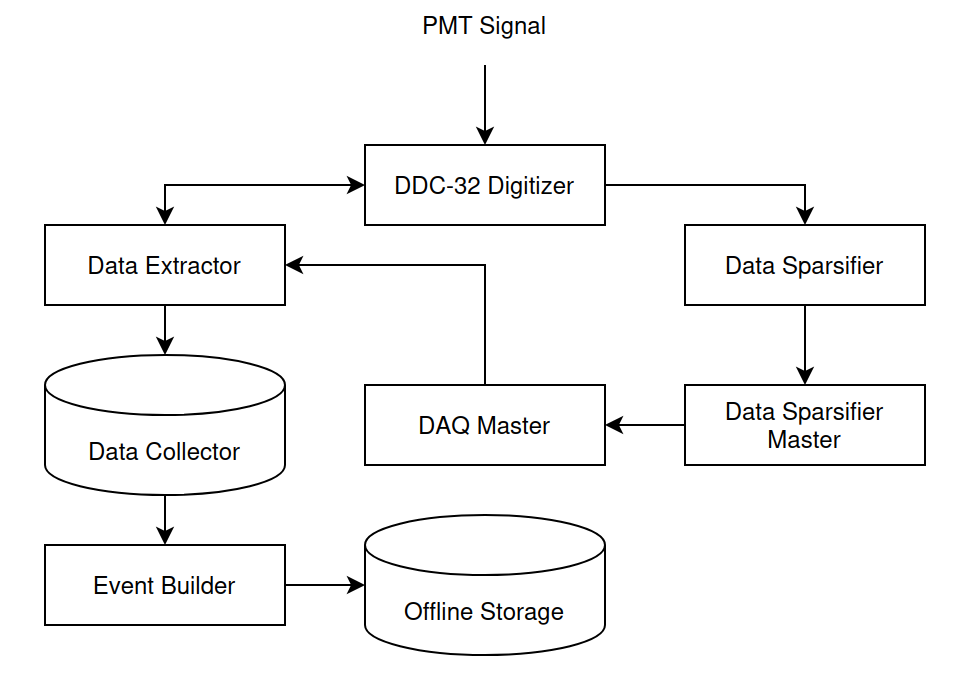
\includegraphics[width=0.7\linewidth]{figures/LZ/LZDAQ.png}
    \caption{A simplified schematic depicting how PMT signals are processed using the LZ DAQ system. Adapted from Ref.~\cite{LZ:2024bvw}.}
    \label{fig:LZ/LZDAQ}
\end{figure}
Results from the POD waveform analysis are passed to the data sparsifiers and grouped by the Data Sparsifier Master (DSM) where a decision is made whether an event has been observed. The DSM informs the DAQ Master and time window is selected for the event and the data is extracted from the digitizers and stored by one of the Data Collectors. A simplified schematic of the LZ DAQ system is shown in \ref{fig:LZ/LZDAQ}, depicting one channel of digital electronics. Event builders take the data which has been temporarily stored on the Data Collectors, organized the data by channel, and assembles full event structures for offline analysis. An in-depth description of FADR can be found at Ref.~\cite{LZ:2024bvw}. 
\section{Simulation techniques}\label{sec:LZ/Simulations}
Simulations of the LZ experiment play a key role understanding the detector and its response. They present several purposes, for example: the calculation of background rates in LZ; the prediction of of sensitivity of the experiment to rare event searches through Profile Likelihood Ratio analysis (PLR); the testing of event reconstruction infrastructure; determining efficiencies of data selection methods. An overview of the LZ simulation framework is shown in \autoref{fig:LZ/LZSimFramework}.
\begin{figure}[!ht]
    \centering
    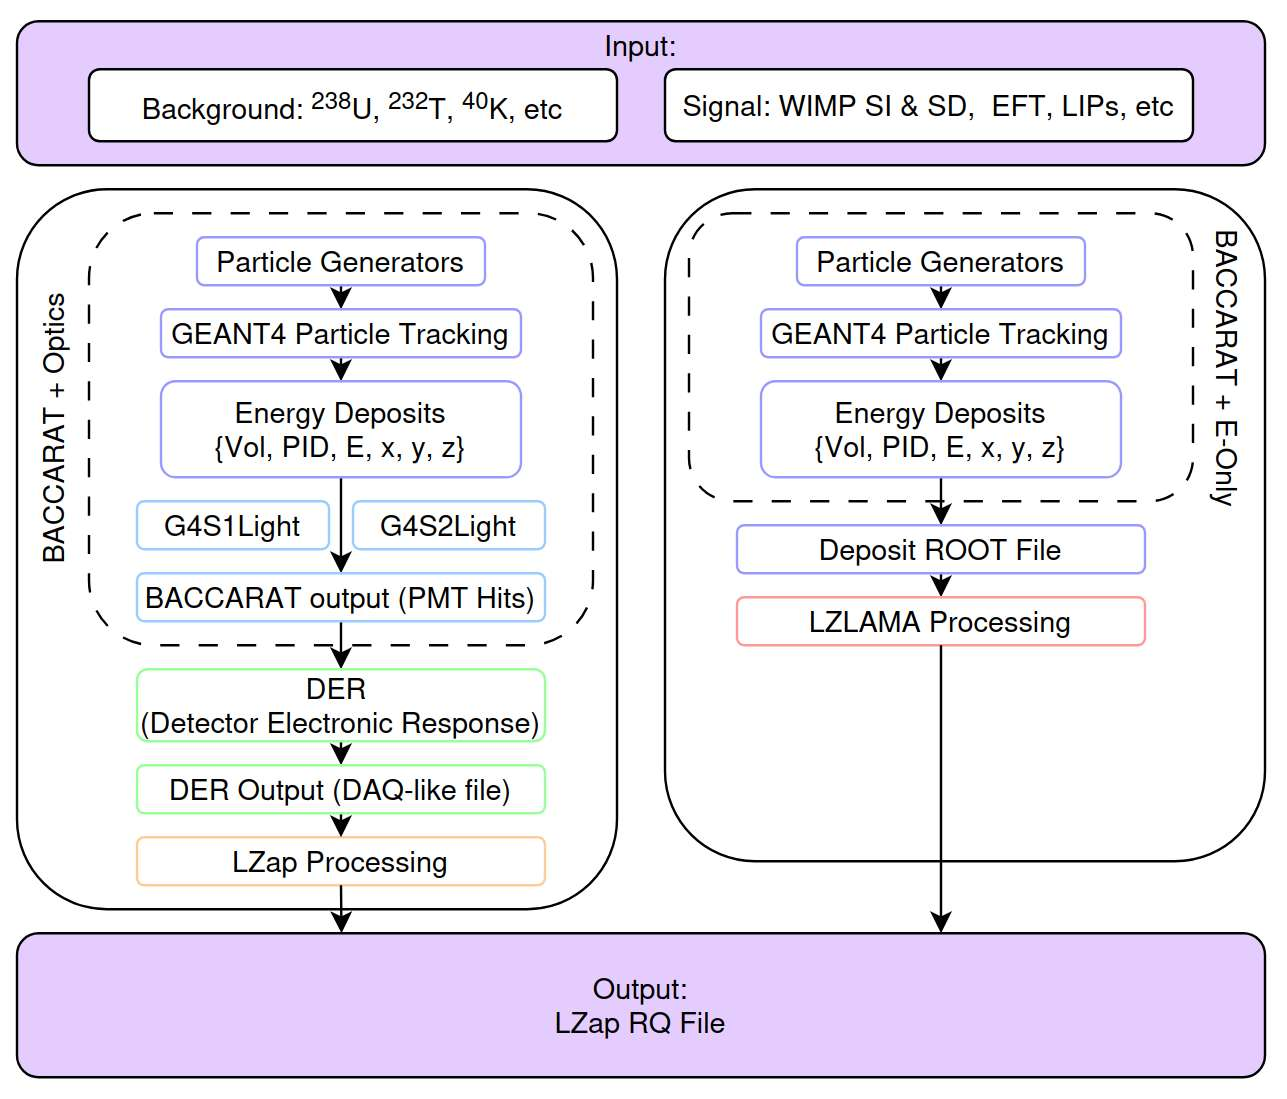
\includegraphics[width=0.95\linewidth]{figures/LZ/LZSimFramework.png}
    \caption{Simulation framework for the LZ experiment. ``Full'' and ``Fast'' simulation chains are shown. Both chains begin with BACCARAT and end with an output LZAP RQ file.}
    \label{fig:LZ/LZSimFramework}
\end{figure}
For all simulations, LZ uses BACCARAT\footnote{\textbf{B}asically \textbf{A} \textbf{C}omponent-\textbf{C}entric \textbf{A}nalogue \textbf{R}esponse to \textbf{A}ny\textbf{T}hing}\cite{LZ_SIMS} package to simulate particle interactions in the detector and this package is built upon the GEANT4 simulation toolkit \cite{GEANT4:2002zbu}. Using GEANT4 along with CAD-Drawing, the LZ experiment is built as a detector geometry. In simulation, a series of inputs can be used to generate particles which are propagated through the detector geometry, with any additional particles being generated from interactions with detector materials. GEANT4 is used to track the particles and identifies the interaction points. From there, two separate chains exist for interpreting this information, \autoref{fig:LZ/LZSimFramework}.

The ``Fast'' chain, seen on the right of \autoref{fig:LZ/LZSimFramework}, records energy deposits in the detector and passes them to LZLAMA for processing. LZLAMA consists of two primary packages, the Noble Element Simulation Technique (NEST) to process interactions in the xenon space and DICEBOX to process interactions with the OD. NEST provides the expected conversion of energy to scintillation photons and ionization electrons based on empirical models developed using experiment measurements \cite{NEST1}. The DICEBOX toolkit is empolyed to handle interactions between neutrons and their capture on Gd as GEANT4 has difficulty conserving Q-value and multiplicity of the gamma emissions from the neutron capture. Energy deposits in other volumes are handled by GEANT4. LZLAMA outputs a ROOT file which has the same reduced-quantity (RQ) format as data processed using LZ's custom processing tool, LZAP \cite{LZ_SIMS}, which performs pulse and event reconstruction.

The second, ``Full'' chain, enables full simulation of optical processes throughout the entire detector including VUV photons and ionisation electrons that are produced in the xenon and scintillation light generated in the OD. Another custom LZ software package, Detector Electronic Response (DER), is used to translate PMT hits in the BACCARAT output into waveforms. The DER simulates the analogue front-end electronics of LZ to produce waveforms, written in an identical format to the true LZ DAQ, \autoref{sec:LZ/LZDAQ}. A number of physical processes are incorporated into the DER to create realistic waveforms including: a PMT response model, gain, quantum efficiency, double photoelectron probability, dynode effects, dark rate, and afterpulsing. This chain is more computationally intensive but it allows for a more realistic, event-by-event analysis. The output from the DER is processed by LZAP to produce RQ-structured files to be analysed much like real data.
A complete review of the LZ Simulation framework can be found at Ref.~\cite{LZ_SIMS}.

\section{Assembly and operation of the LZ detector}\label{sec:LZ/LZAssembly}
During the past six years whilst the author has collaborated on the LZ Experiment, a significant portion of that time has been spent on-site at SURF working on the assembly, commissioning and operation of the LZ Detector. These efforts began with the installation of the OCS electronics and an in-situ-calibration of the LED system in November 2019, this work is detailed extensively in Ref.~\cite{hbirch:thesis}. Photographs of the author with an OCC and working in the OCS rack are shown in \autoref{fig:LZ/OCSInstall}.

\begin{figure}[ht!]
    \centering
    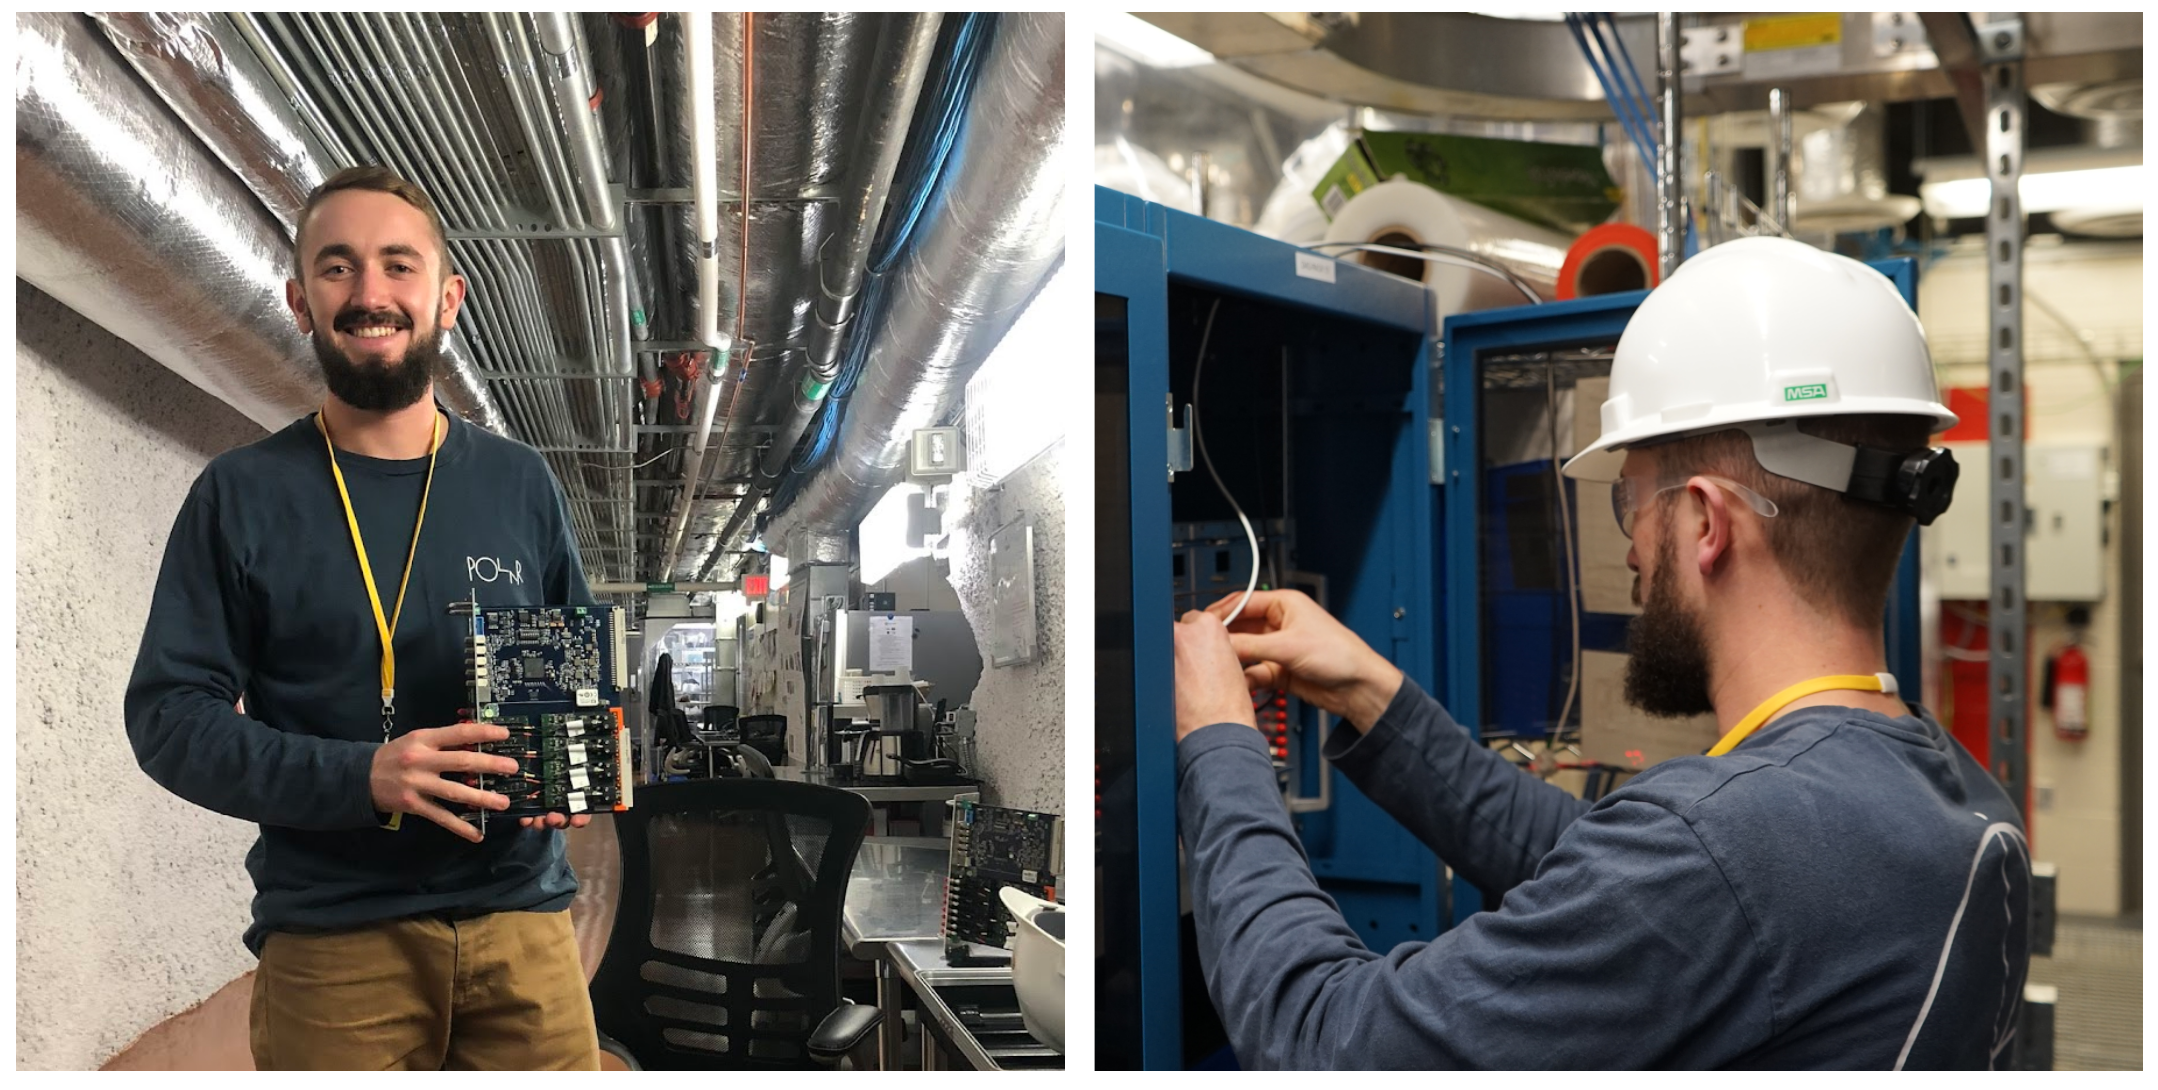
\includegraphics[width=0.9\linewidth]{figures/LZ/OCSInstall_2panel.png}
    \caption[OD OCS electronics installation.]{OD OCS electronics installation. \textbf{Left:} The author standing in the common corridor at the Davis Campus holding an OCC prior to the OCS electronics installation. \textbf{Right:} The author making serial connections between the front planes of the OCS OCCs within the electronics racks.}
    \label{fig:LZ/OCSInstall}
\end{figure}

The construction of the OD PMT system and OCS fibre installation took place between November 2020 and April 2021. A photograph of the complete OD PMT system prior to filling is shown in \autoref{fig:LZ/ODImg}, alongside a photograph of the six person OD PMT system installation team. The OD PMTs are visible which are attached to a stainless steel support structure (faintly outlined by shadow in \autoref{fig:LZ/ODImg}). Tyvek covers the support structure, DD conduits, OCV and cathode high voltage (HV) umbilical to increase light collection efficiency of the OD. The author was responsible for the completion of the OD PMT installation, managing the HV and signal cable routing operation. A total of 6~km of cable was routed from the PMTs in the water tank to the DAQ electronics racks situated on the upper level of the Davis Cavern. The final cable routing of the all 120 PMTs to their respective power supplies and amplifiers is shown in the left panel of \autoref{fig:LZ/Gonk2}.

\begin{figure}[ht!]
    \centering
    \includegraphics[width=\textwidth]{figures/LZ/Screenshot from 2025-07-22 19-21-29.png}
    \caption[Completed Outer Detector prior to filling in May 2021 alongside OD PMT installation team.]{\textbf{Left:} Completed Outer Detector prior to filling in May 2021. \textbf{Right:} OD PMT installation team, M. Williams (bottom right), A. Rodriguez (bottom left), L. Korley (middle right), D. Lucero (middle left), J.J. Wang (upper right), and author (upper left). Photographs used with permission from M. Kapust.}
    \label{fig:LZ/ODImg}
\end{figure}

Due to the COVID-2019 pandemic\footnote{Due to travel restrictions the group from the University of Liverpool where unable to travel to SURF to assist the author with the installation.} the author was entirely responsible for installing the OCS fibre system and monitoring PMT, a photograph of the author holding the monitoring PMT is shown in the middle panel of \autoref{fig:LZ/Gonk2}. The commissioning of the OD PMT system and OCS followed in May 2021 with all PMTs and OCS injection points operating as expected.

\begin{figure}[ht!]
    \centering
    \includegraphics[width=\linewidth]{figures/LZ/GonkThreepanel.png}
    \caption{The author and the fruits of many labours. \textbf{Left:} Final OD HV and Signal cable routing viewed from the rear of Rack 9. \textbf{Middle:} A photograph of the author holding the OD OCS monitoring PMT prior to its installation into the rack mounted dark box below the OCS electronics, \textit{YNWA}. \textbf{Right:} The author sporting a dashing PPE set whilst dispensing nitrogen to cryopump the source injection panel prior to a flow through source calibration.}
    \label{fig:LZ/Gonk2}
\end{figure}

From April 2023 - August 2024, the author was a member of the on-site scientific support team at SURF. The role covered many different tasks to ensure LZ remained operational, from managing the deployment of rod sources during calibration campaigns to maintenance of detector subsystems such at the OD water circulation system. A photograph of the author dispensing liquid nitrogen whilst cryopumping the source injection panel is shown in right panel of \autoref{fig:LZ/Gonk2}.

\iffalse
In addition to the analyses detailed in the following chapters, the author has fulfilled key roles on the experiment:
\begin{itemize}
    \item OD Optical Calibration Lead/Expert \textit{(2019 - 2025)}
    \item OD PMT Expert \textit{(2021 - 2025)}
    \item PMT Shift Supervisor \textit{(2021 - 2025)}
    \item On-site science support \textit{(April 2023 - August 2025)}
    \item Deputy Outer Detector Coordinator \textit{(April 2023 - December 2024)}
    \item Supervised Black Hills State University undergraduate student through the DoE SC-RENEW program \textit{(September 2023 - July 2024)}
\end{itemize}
\fi